\hypertarget{results}{\section{Analysis}}
\label{sec:results}

The finalized results of the \projectname are the scores for each of the \numindicators indicators across all \numcompanies companies.
These result are accessible at \materialsUrl, to facilitate subsequent analyses.
Here, we specifically consider overarching trends in the results, along with more specific trends based on the structure of the index.
Namely, we analyze along the rows/indicators (\eg domains), the columns/companies (\eg release strategy), as well as data-driven trends (\eg correlations).

\hypertarget{overarching-results}{\subsection{Overarching results}}
\label{sec:overarching-results}

\begin{figure}
\centering
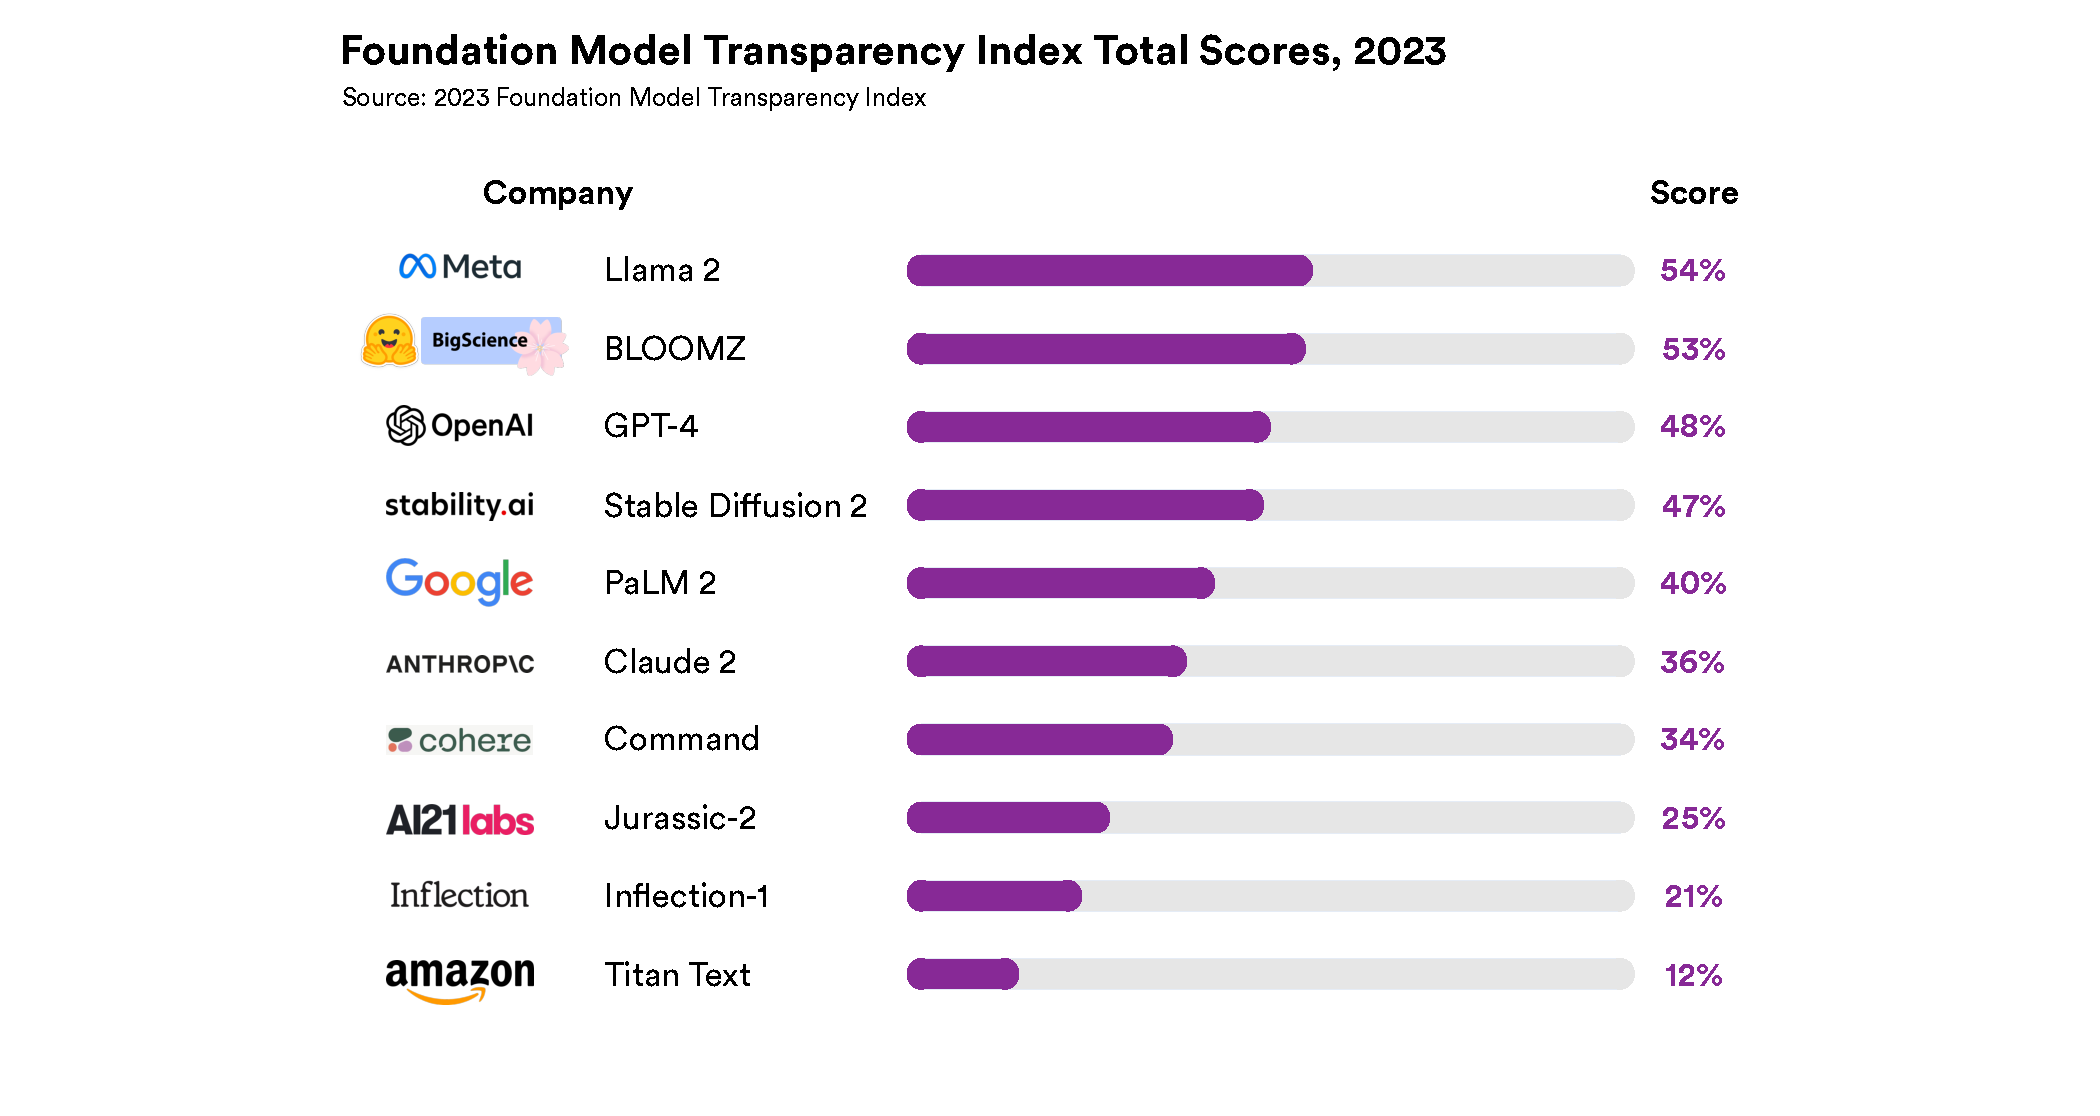
\includegraphics[keepaspectratio, height=\textheight, width=\textwidth]{figures/f7.pdf}
\caption{\textbf{Overall Scores.} The overall \projectname score and ranking across all \numindicators indicators.}
\label{fig:overall-scores}
\end{figure}

\begin{figure}
\centering
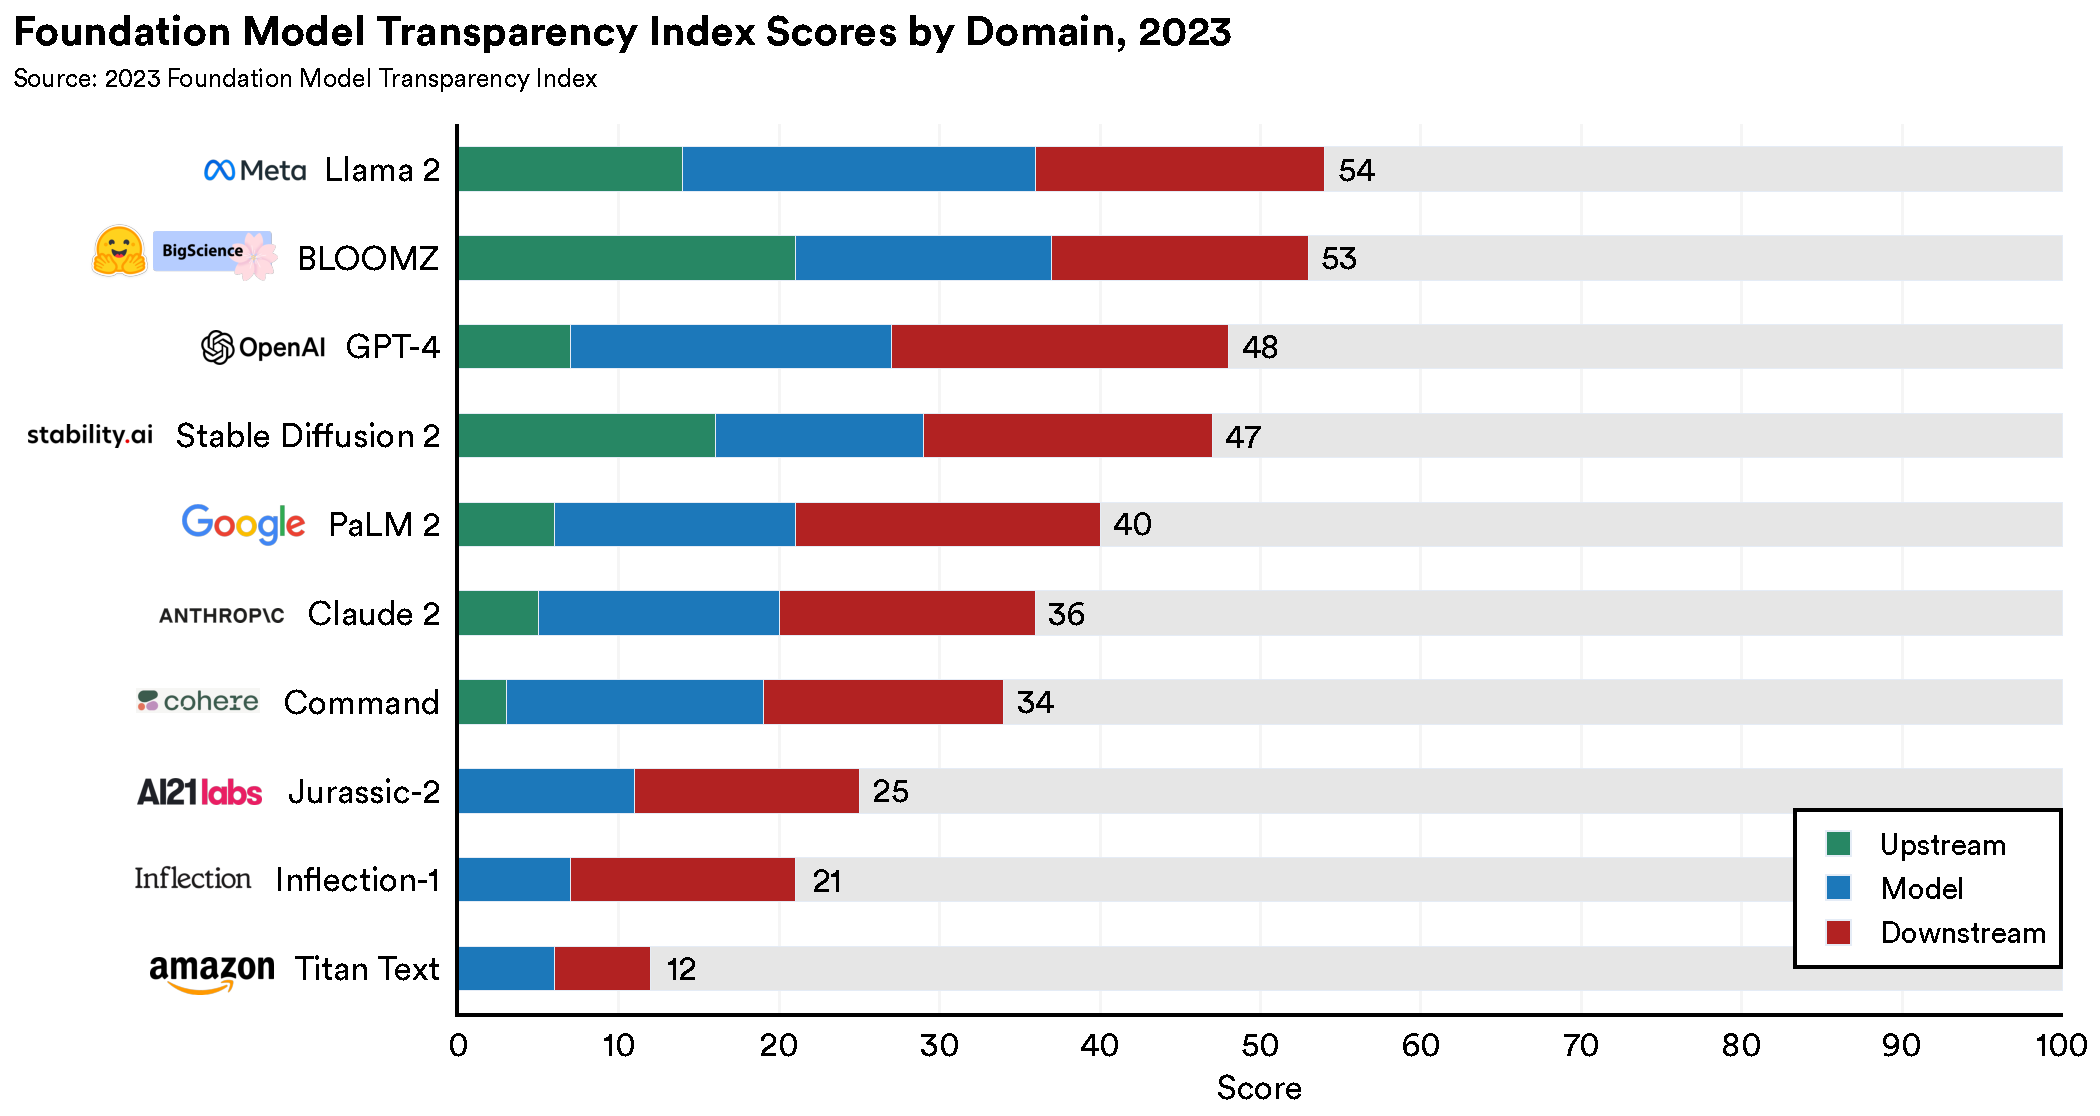
\includegraphics[keepaspectratio, height=\textheight, width=\textwidth]{figures/f8.pdf}
\caption{\textbf{Scores by Domain.} The aggregate score of each developer broken down by the three domains: upstream, model, and downstream.
}
\label{fig:domain-scores}
\end{figure}

\begin{figure}
\centering
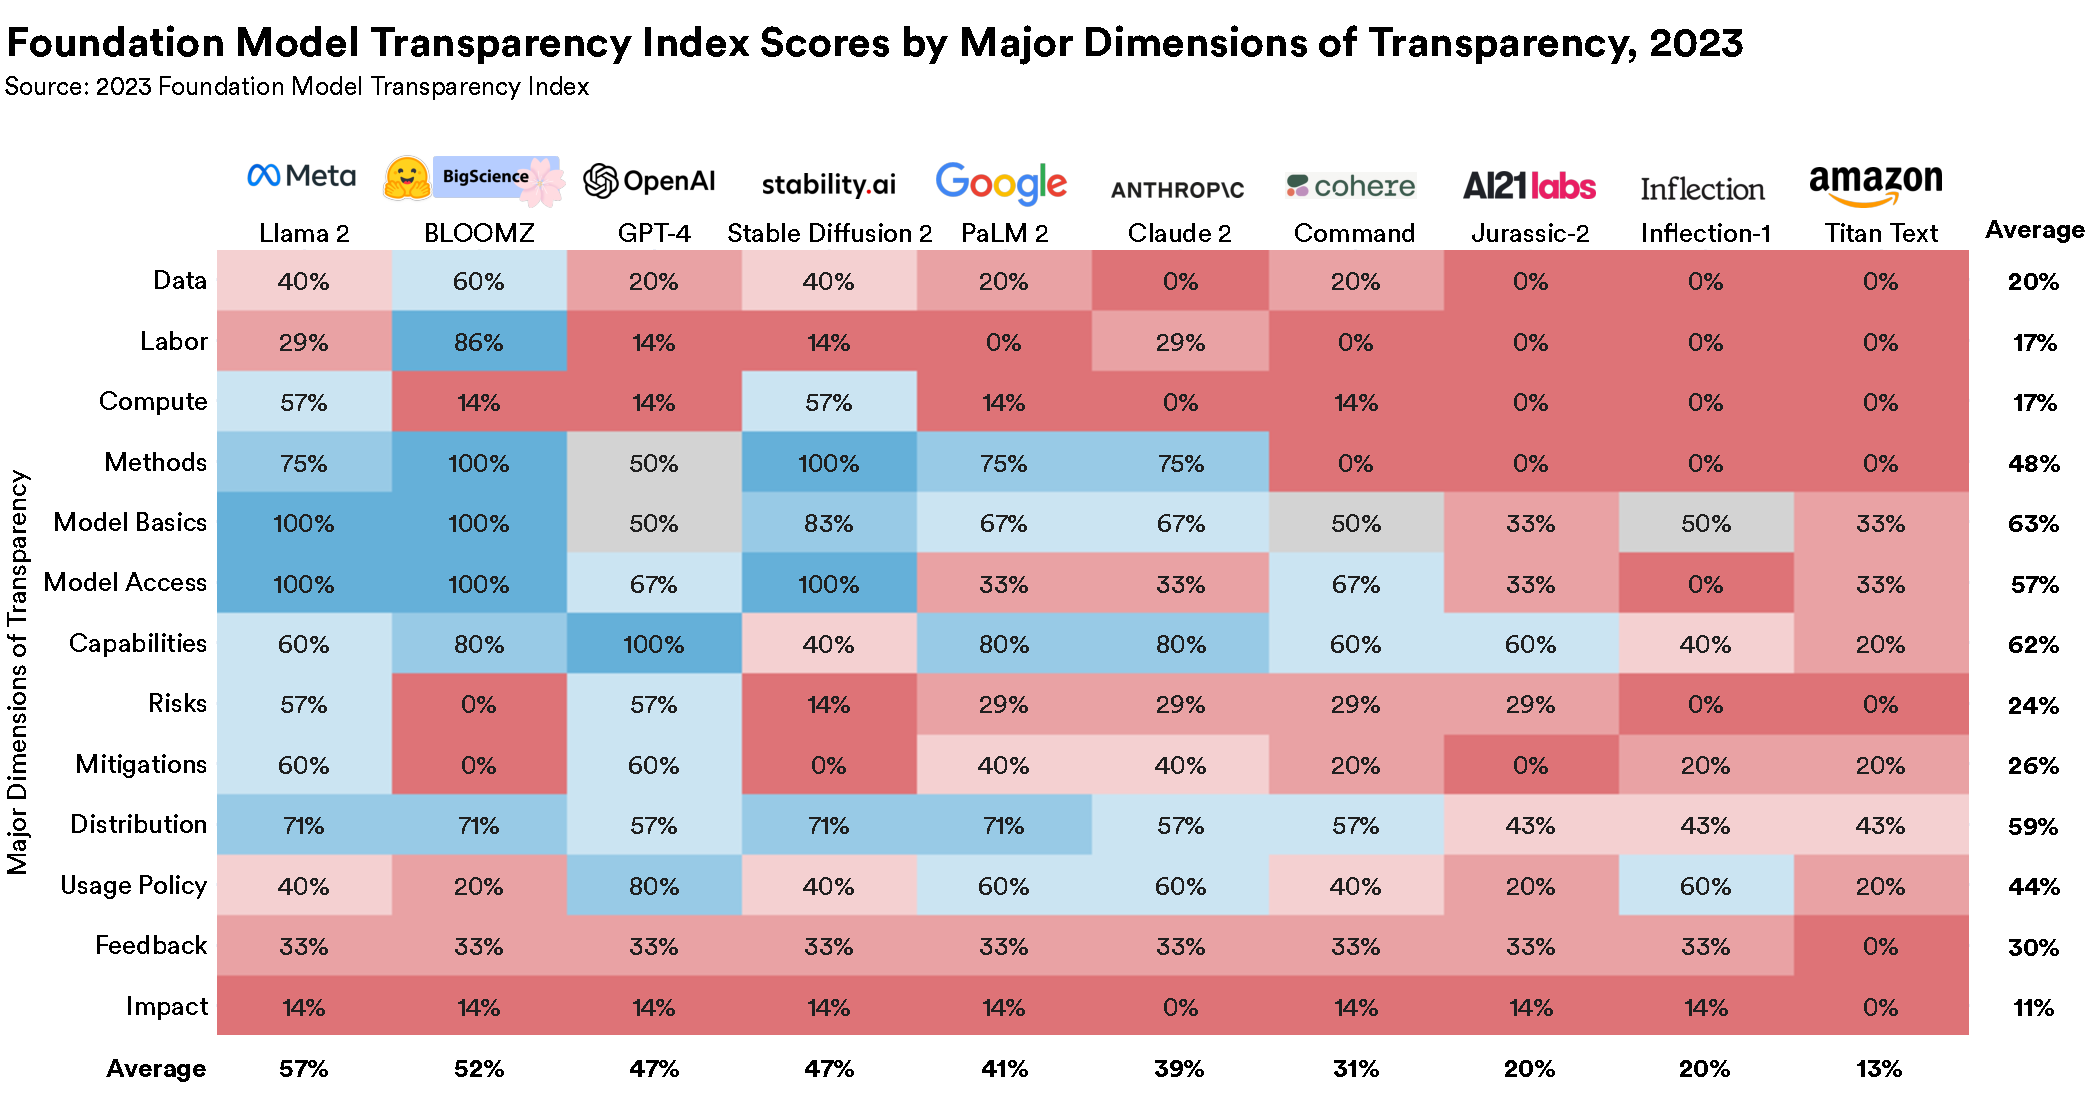
\includegraphics[keepaspectratio, height=\textheight, width=\textwidth]{figures/heatmap_selected_subdomains.pdf}
\caption{\textbf{Scores by Major Dimensions of Transparency.} 
The fraction of achieved indicators in each of the \nummajorsubdomains major dimension of transparency. 
Major dimension of transparency are large subdomains within the \numsubdomains subdomains.}
\label{fig:major-subdomain-scores}
\end{figure}

We begin our analysis by first establishing the broad trends when viewing the index as a whole.
We consider results aggregated at the level of a single overall score per company (\reffig{overall-scores}) as well as the scores broken down into the \numdomains domains (upstream, model, downstream; \reffig{domain-scores}).
We supplement our findings on these overarching trends with a more granular consideration of the \textit{major dimensions of transparency} in the index in \reffig{major-subdomain-scores}.\footnote{
The major dimensions of transparency we highlight are \nummajorsubdomains large subdomains among the \numsubdomains subdomains. }


\paragraph{All developers have significant room for improvement. But most transparency indicators are very obtainable, having been implemented by at least one developer.}
Based on \reffig{overall-scores}, the highest-scoring developer scores points for \maxscore of the \numindicators indicators, and the average score across all developers is \meanscore.
This establishes a pervasive lack of transparency across major foundation model developers.
With that said, for \numfeasible of the \numindicators indicators, there exists some developer that scores points, and of these there are \numfeasiblemultiple where multiple developers score points. 
Consequently, there is clear reason to believe that across all developers, the necessary change to become more transparent is feasible.
That companies' competitors are more transparent in certain issue areas suggests that such transparency, even if not fully costless, is unlikely to cause serious damage to their business.
Companies can emulate the higher level of transparency their competitors exhibit on certain indicators, providing a precedent and a starting point for improving transparency in the foundation model ecosystem. 

\paragraph{Developers show significant variance in overall transparency scores.}
While all developers have significant room for improvement, the current transparency of developers is strikingly uneven. 
Namely, the range in overall scores is \scorerange between the highest-scoring \meta at \maxscore and the lowest-scoring \amazon at \minscore.
Even excluding \amazon's score as especially low, we still see an effective range of 30 points between \meta and the next lowest \inflection.
Overall, with respect to the mean of \meanscore, the standard deviation is \stdev, which is quite substantial.
The four top-scoring developers (\meta, \huggingface, \openai, \stability) all cluster well above the mean, the next three are very close to the mean (\google, \anthropic, \cohere), and the three lowest-scoring developers (\aitwentyone, \inflection, \amazon) are well below the mean.
In many cases, the lowest-scoring developers have clear opportunities for improvement through straightforward changes related to some of the least challenging indicators. 
Examples include improved documentation(\eg change logs, versioning protocols, model cards, centralized documentation for downstream use), clearer language in corporate policies(\eg usage policies, model behavior policies, deprecation policies), and disclosing additional information that is unlikely to have implications for business competitiveness or safety (\eg basic details on methods, dependencies, feedback).

\paragraph{The Upstream domain sees the worst transparency scores.}
To gain additional insight beyond developers' basic overall scores, we consider scores broken down by the \numdomains top-level domains in \reffig{domain-scores}.
On this basis, we see clear evidence that developers are, on average, least transparent with respect to the upstream resources required to build their models, such as data, labor, and compute. 
Concretely, the mean score on upstream indicators is 7.2 out of 32 (22.5\%), compared to 14.1 out of 33 (42.7\%) for model indicators and 15.7 out of 35 (44.9\%) for downstream indicators.
To confirm this is not overly biased by outliers, we note that the medians show the same trend: the median score on upstream indicators is 3.5, compared to 12.5 for model indicators and 16 for downstream indicators.
We specifically highlight that the four lowest-scoring developers overall (\reffig{overall-scores}) also fare the worst on the upstream domain (\reffig{domain-scores}), with \cohere receiving 3 points and all of \aitwentyone, \inflection, and \amazon receiving 0 points.
In contrast, for both the model and downstream domains, all \numcompanies companies receive at least 6 points. 

\paragraph{Domain-level discrepancies explain some of the differences between companies with similar overall scores.}
We partition the \numcompanies companies into three groups based on whether their overall score (\reffig{overall-scores}) is well-above (\meta, \huggingface, \openai, \stability), around (\google, \anthropic, \cohere), or well-below (\aitwentyone, \inflection, \amazon) the mean. 
Within these groups, while companies receive somewhat similar scores, we find that their domain-level scores clarify discrepancies between them. 
Among the highest scorers, \openai is considerably less transparent on upstream matters (7) as compared to the other three high-scoring companies (\meta with 14, \huggingface with 21, \stability with 16).
In particular, \openai and \stability receive the nearly the same overall score, with \openai making up the deficit to \stability on upstream transparency mostly through better model-level transparency (and, specifically, many of the indicators on evaluations and risks).
For the middle category of \google, \anthropic, and \cohere, the discrepancies are less stark, but we do see that \cohere is at 3 in the upstream category compared to \google with 6 and \anthropic with 5.
Given the broadly similar scores for these three developers across all of the domains, we revisit the extent to which they are correlated at a finer-grained level in \refsec{correlations}.
Among the three lowest-scoring developers, we see that \aitwentyone and \inflection are differentiated by the model domain, with both scoring a zero on the upstream domain and similarly on the downstream domain.

\paragraph{\data, \labor, and \compute are pervasive blind spots across developers.} 
While the overall and domain-level results provide a basic lay of the land, we find that the major dimensions of transparency provide the Goldilocks region for clear and incisive analysis as shown in \reffig{major-subdomain-scores}.
In particular, these dimensions of transparency are subdomains with several indicators (so the subdomain scores are more reliable) that are tied to broadly-understandable concepts like labor and capabilities. 
We hone in on the following major dimensions of transparency: \data, \labor, \compute, \methods, \modelbasics, \modelaccess, \capabilities, \risks, \modelmitigations, \distribution, \usagepolicy, \modelbehaviorpolicy, \updates, \dataprotection, \feedback, and \impact. 
Analysis at this level reveals actionable insight into what types of transparency or opacity lead to many of our top findings. 
For example, we find that the poor upstream transparency stems from low performance on the \data, \labor, and \compute subdomains; developers average just 20\%, 17\%, and 17\% for \data, \labor, and \compute respectively. 
In terms of smaller subdomains, developers on average score 25\% of the available points on \datamitigations.

\paragraph{\modelbasics, \capabilities, \limitations, and \dataprotection are the most transparent subdomains at present, but still short of the ideal.}
Developers score the highest proportion of points on indicators related to the following subdomains: \interface (85\%), \documentation (70\%), \dataprotection (67\%), \modelbasics (63\%), and \updates (63\%).
This reflects some baseline level of transparency across developers with respect to notifying users they are interacting with AI systems, providing centralized documentation for downstream use, publishing data protection policies, and disclosing the modalities associated with their model. 
Still, there are gaps in even for these subdomains. 
No developer provides a protocol for accessing usage data.
Most developers (8 of 10) do not disclose the size of their model.
And only half of the developers provide any form of deprecation policy.

\hypertarget{upstream-results}{\subsection{Upstream results}}
\label{sec:upstream-results}

Upstream indicators assess transparency regarding the ingredients that go into the foundation model including data, labor, compute, methods, and code. 
These ingredients are important predictors of the capabilities and risks of the foundation model they produce, as well as externalities of the model development process (\eg impacts on human laborers and the environment). 
As we show in \reffig{domain-scores}, the upstream indicators are the most sparsely awarded (22.5\% coverage on average).
Here, we analyze at the level of subdomains and indicators based on \reffig{upstream-scores}. 

\paragraph{The Upstream domain shows the greatest spread.}
Building on the fact that developers score worst on the upstream domain--with several developers scoring exactly or nearly 0 points--we find the range in scores is the greatest for this domain. Namely, only one developer (\huggingface) scores more than half of the indicators (21 of the available \numupstreamindicators indicators; 65.6\%), yielding a range of 21 when compared to the lowest-scoring developers: \aitwentyone, \inflection, and \amazon (0 of the available \numupstreamindicators indicators; 0\%).
We emphasize this striking disparity given that many of the fundamental societal issues in connection with foundation models relate to upstream resources: bias, copyright, and privacy in relation to data, worker protections and fair compensation in relation to labor, environmental impact and energy expenditure in relation to compute, reproducibility in relation to methods, and cybersecurity in relation to code. 

\paragraph{The \methods subdomain is the most transparent in aggregate, while \labor is the least transparent.} 
Among the upstream subdomains, only \methods shows some degree of coverage, with six of the developers giving some description of training stages, training objectives, and dependencies.
On the other end of the spectrum, \labor sees little to no coverage with the exception of \bloomz, which involved volunteers providing data.
Developers generally share no information about the use of human labor in their data pipeline, the employer, wages, and geographical distribution of these workers, instructions they give to data annotators, or any labor protections they implement.
This industry norm of being nontransparent with respect to data labor is in tension with the fact that such information is critical to reinforcement learning with human feedback \citep{ziegler2019finetuning, ouyang2022instructions, casper2023open}.
That data labor is one of the two least transparent subdomains is consistent with prior work documenting widespread ethical challenges with data labor \citep{gray2019ghost, crawford2021atlas, hao2023cleaning}. 

\paragraph{The \compute subdomain shows major discrepancies among developers.} 
\meta and \stability document some aspects of compute, energy, and hardware usage, as well as the carbon footprint of model development, whereas many developers do not. 
Given the significant compute expenditure required to build many foundation models, the practice of documenting energy use and environmental impact is well-established along with associated tooling to measure these quantities \citep{lacoste2019quantifying,strubell2019energy,schwartz2020green,luccioni2023counting}. 
In spite of this, most developers do not disclose minimal, or sometimes any, details related to compute usage, particularly with respect to energy usage, carbon footprint, and environmental impact.

The broader environmental impact of building foundation models is also essential to consider; although there has been significant public attention concerning energy expenditure, other matters such as water usage may be of similar consequence environmentally \citep{luccioni2023counting}.
\citet{luccioni2022estimating} provides an excellent example, documenting the embodied emissions, dynamic consumption, and idle consumption associated with BLOOM \citep{scao2022bloom}.
Given that \bloomz is derived from BLOOM, we note the potential for \textit{documentation transience}, where prior documentation is not updated to reflect substantial changes and, therefore, does not correctly persist to the new asset. 
In particular, the additional broader environmental impact of deriving \bloomz from BLOOM is not disclosed.

\paragraph{Widespread lack of upstream transparency on data creators, data license, copyrighted data and associated mitigations, and broader environmental impact.} 
Of the \numupstreamindicators indicators, no company scores points on six of them.
These are the indicators for data creators, data license status, copyrighted data, copyright mitigations, compute usage and broader environmental impact.
For data creators, in part we believe this reflects the nascent status of methods for providing web-scale understanding of who created the data (\eg text, images) scraped from the Internet. 
However, we recognize that \huggingface in particular has taken important steps to characterize aspects of who created the data, along with associated metadata for copyright, license, and personal information, for the ROOTS corpus used to build BLOOM (though not the additional data involved in building \bloomz). 
With respect to the copyrighted data and data license status indicators, we emphasize that information related to these indicatorsis at issue in ongoing litigation. 
In particular, \stability has explicitly argued that training foundation models on copyrighted data is protected by fair use doctrine in the U.S.\footnote{See \url{https://www.judiciary.senate.gov/imo/media/doc/2023-07-12_pm_-_testimony_-_brooks.pdf} and \url{https://www.documentcloud.org/documents/23589439-openai-motion-to-dismiss} as well as \citet{lemley2020fair}.} 
Closed developers may also view information related to their data as a key competitive advantage, or be disincentivized to share this information due to a perception of legal risk.
Additionally, we note that we are surprised no developer directly discloses the compute usage in FLOPs to sufficient precision, though several disclose information that could be used to compute an estimate or upper bound. 

\edef\originalwidth{\the\pdfpagewidth}
\edef\originalheight{\the\pdfpageheight}




\eject
\pdfpageheight=\originalwidth
\newlength{\mylength}
\setlength{\mylength}{\originalheight-3.4cm}
\pdfpagewidth=\mylength
\newgeometry{margin=1.7cm}

\begin{figure}
\begin{minipage}{\pdfpagewidth}
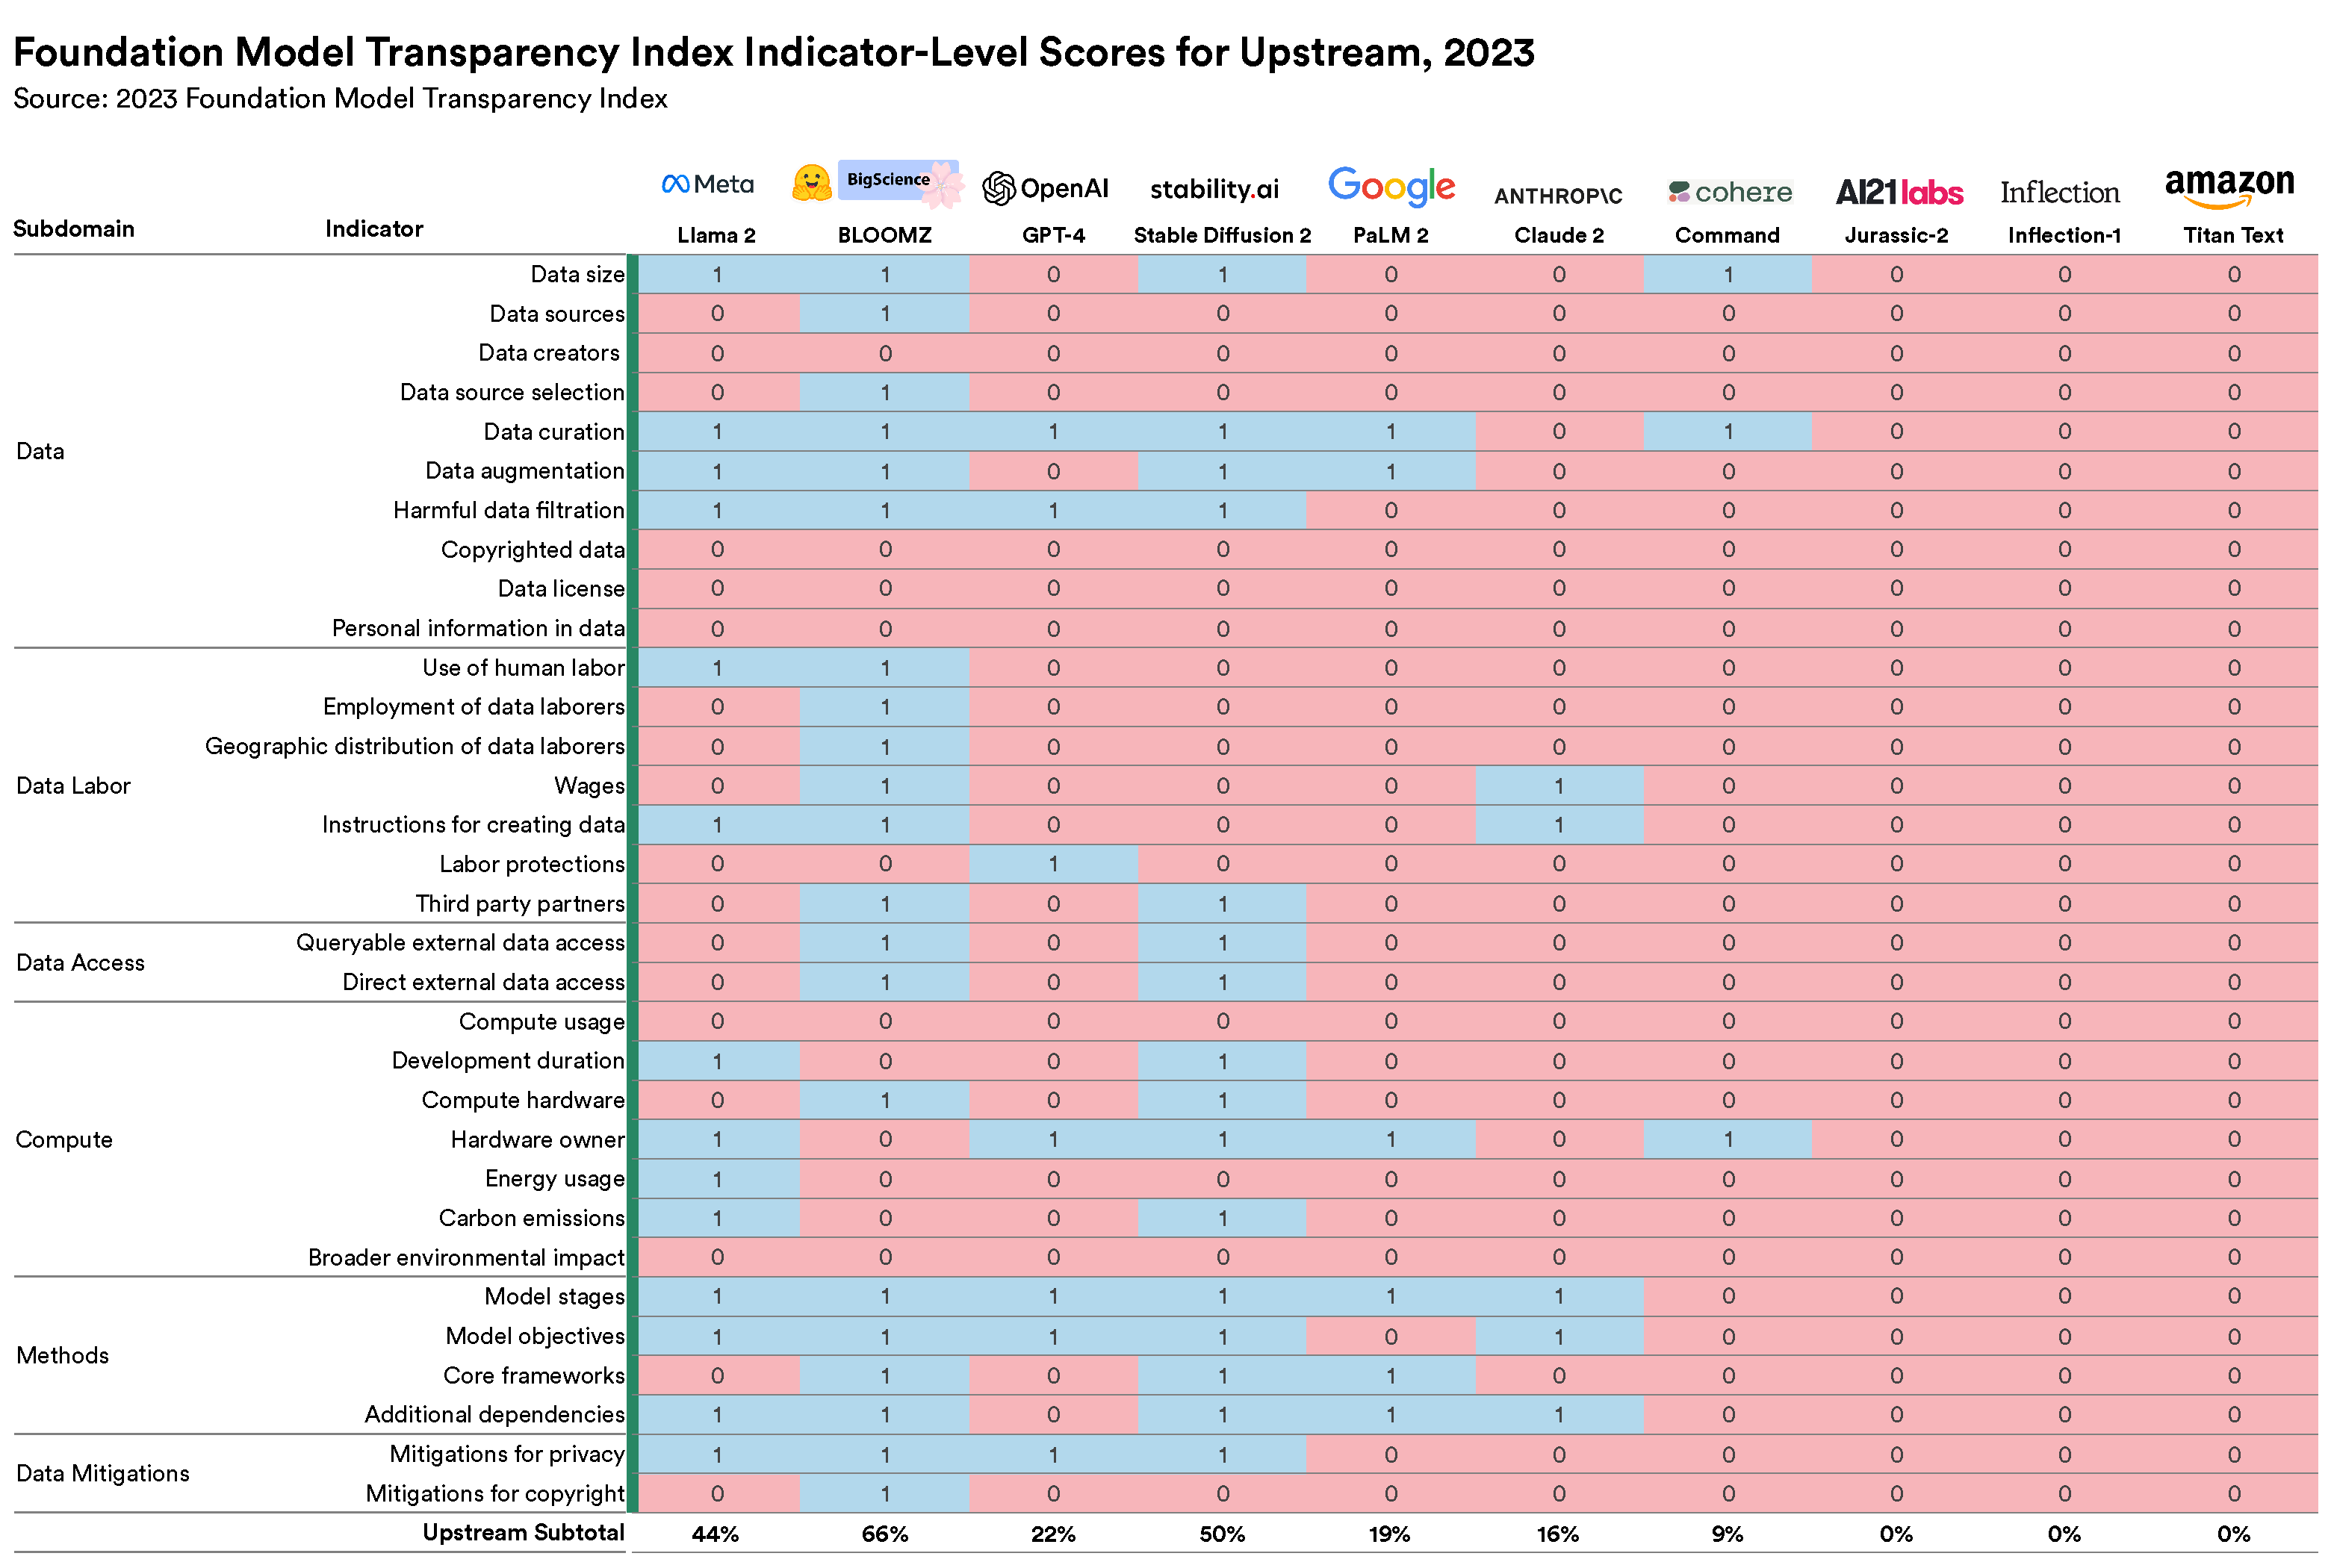
\includegraphics[keepaspectratio, width=0.85\pdfpagewidth]{figures/f10.pdf}
\end{minipage}
\caption{\textbf{Upstream Scores by Indicator.} The scores for each of the \numupstreamindicators upstream indicators.
}
\label{fig:upstream-scores}
\end{figure}

\clearpage

% Revert to initial values
\eject
\pdfpagewidth=\originalwidth \pdfpageheight=\originalheight
\newgeometry{top=2cm, head=10pt, left=2cm, right=2cm,bottom=2cm}



\eject
\pdfpageheight=\originalwidth
\setlength{\mylength}{\originalheight-3.4cm}
\pdfpagewidth=\mylength
\newgeometry{margin=1.7cm}

\begin{figure}
\begin{minipage}{\pdfpagewidth}
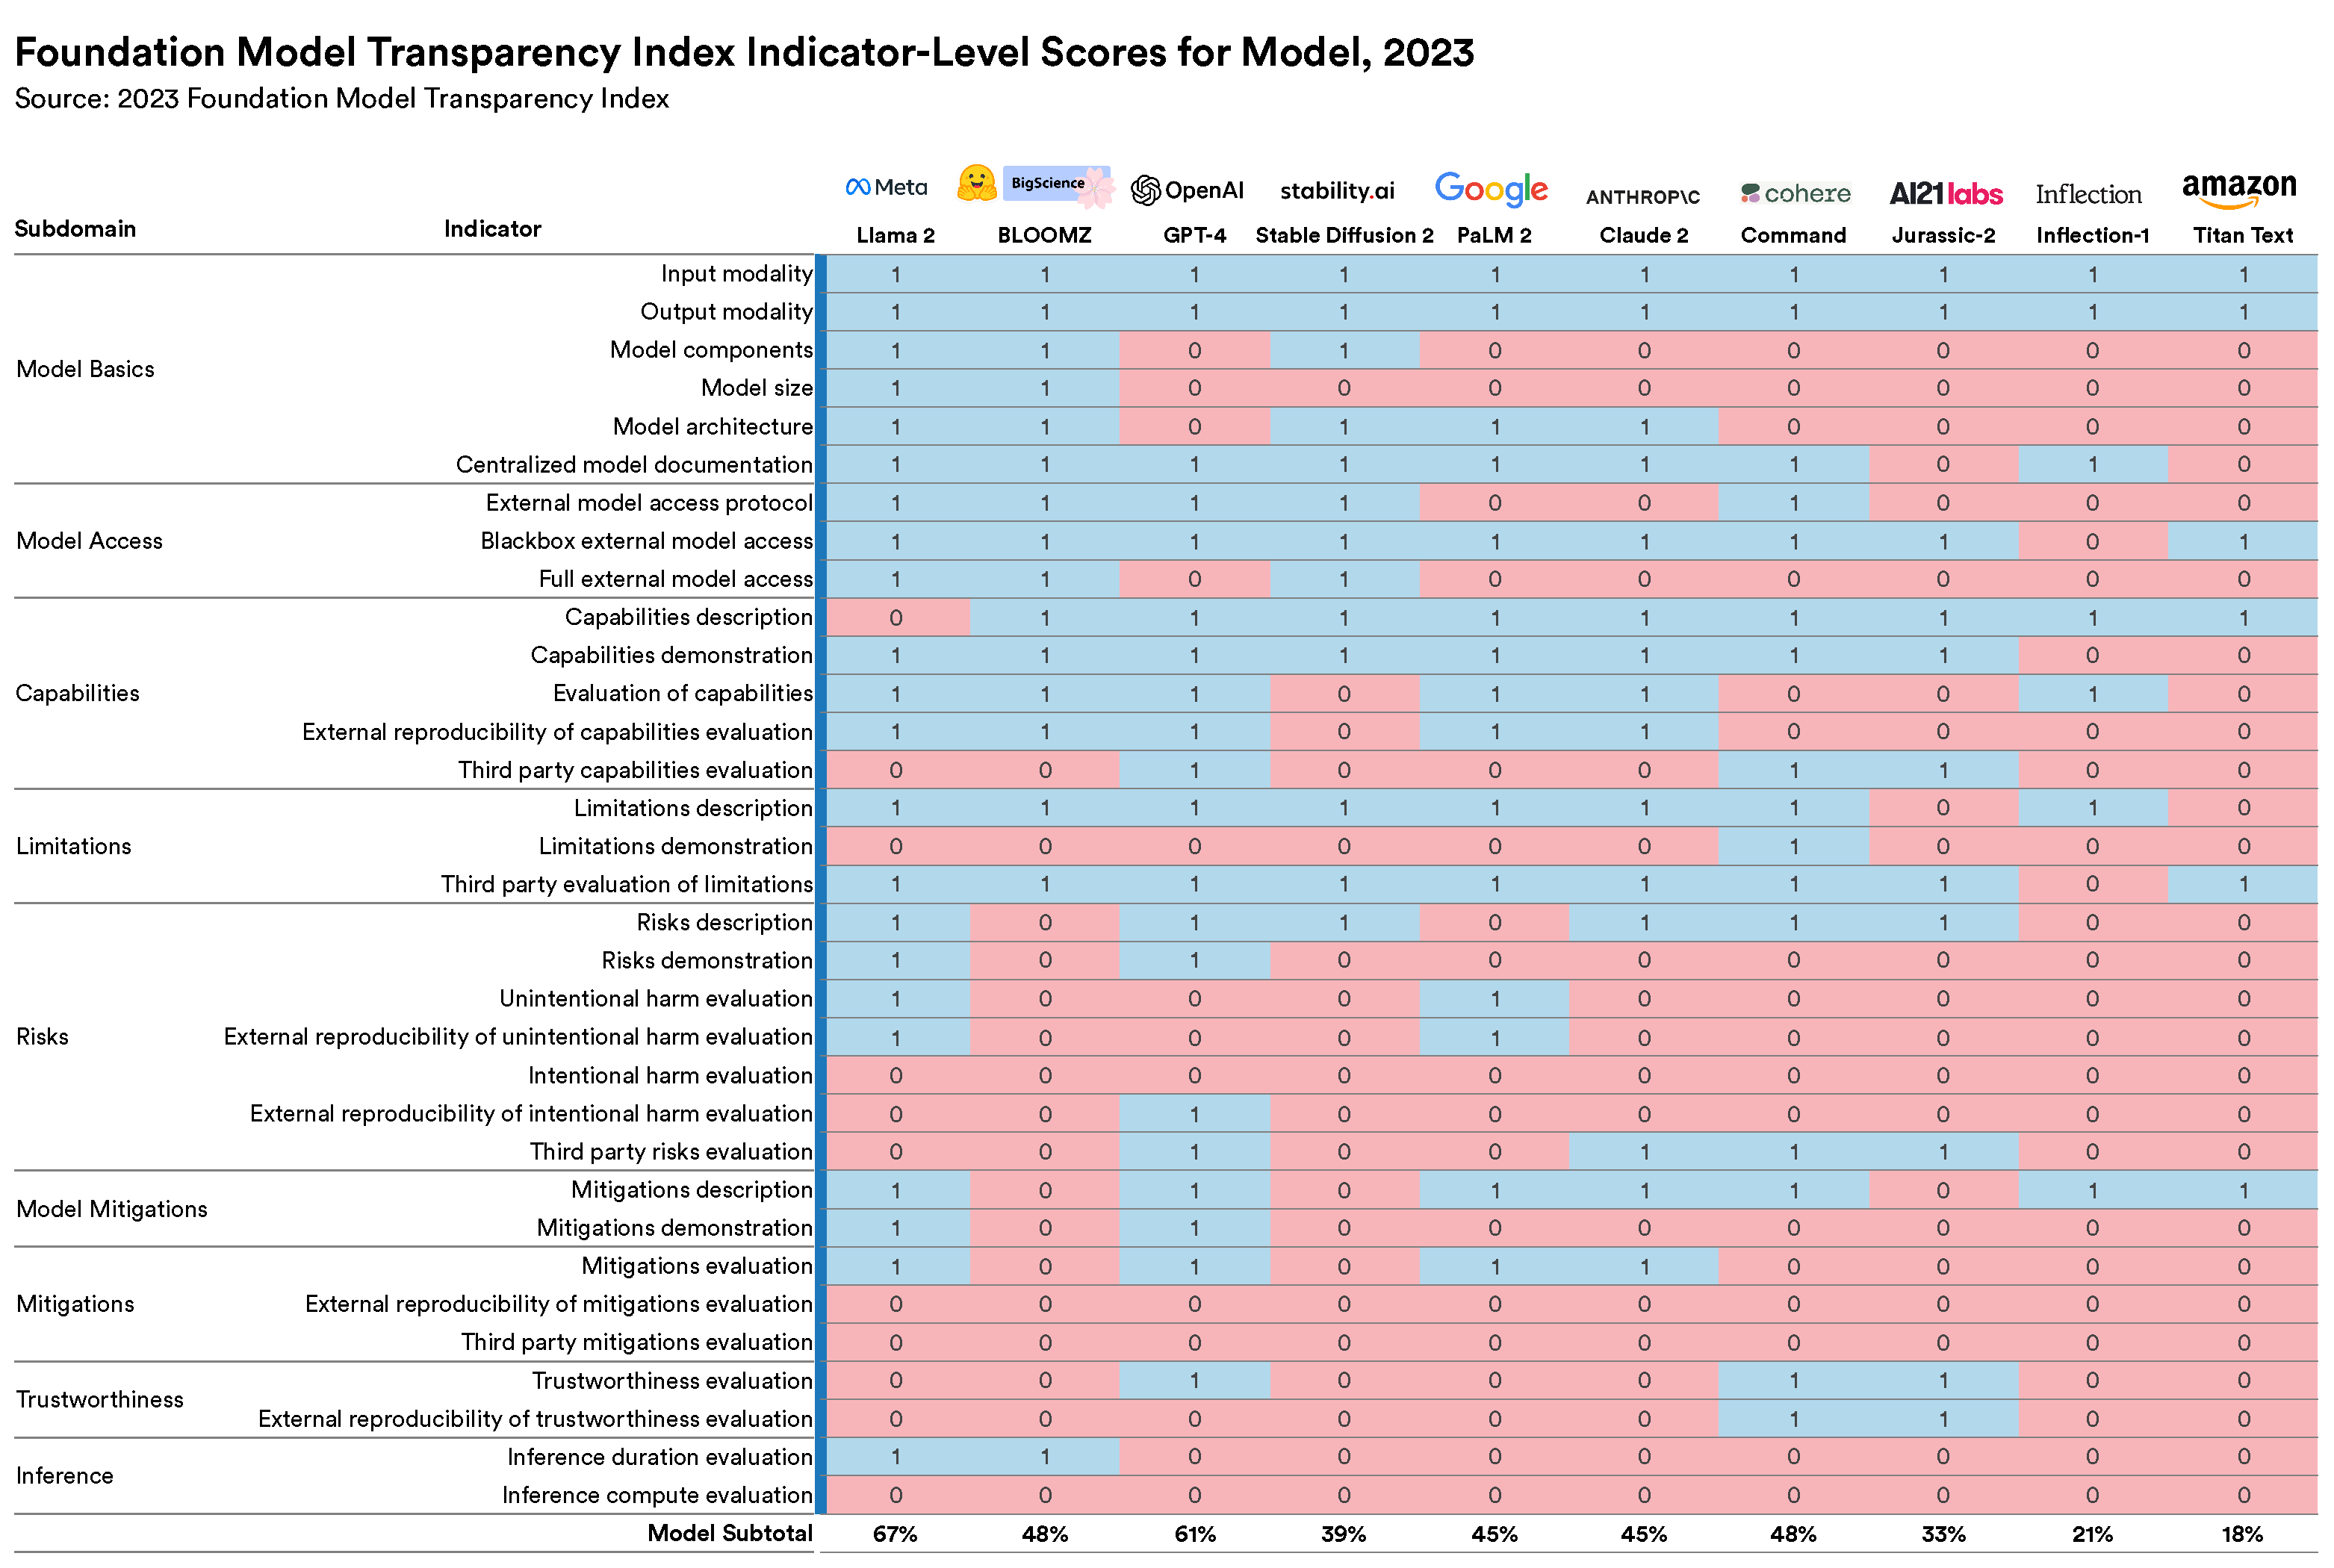
\includegraphics[keepaspectratio, width=0.85\pdfpagewidth]{figures/heatmap_allindicators_model-1.pdf}
\end{minipage}
\caption{\textbf{Model Scores by Indicator.} The scores for each of the \nummodelindicators model indicators.
}
\label{fig:model-scores}
\end{figure}

\clearpage

% Revert to initial values
\eject
\pdfpagewidth=\originalwidth \pdfpageheight=\originalheight
\newgeometry{top=2cm, head=10pt, left=2cm, right=2cm,bottom=2cm}


\paragraph{No upstream indicators are satisfied by all developers.}
At the indicator level, there is no upstream indicator for which every developer receives points.
Of course, this is guaranteed by the presence of (multiple) developers that score 0 points on the entire upstream domain.
Even putting these 3 developers aside, there is no indicator that is satisfied by all of the remaining 7.
The indicators where the greatest number of developers score points are data curation (all but \anthropic) and model stages (all but \cohere), which both suggest that developers are generally willing to describe the basics of the overall pipeline of model development.
With that said, we take the absence of any upstream indicator where all companies score points, and the fact that 5 or more developers score no points on 30 of \numupstreamindicators upstream indicators, as strong evidence that upstream transparency is the domain with the broadest room for improvement.

\hypertarget{model-results}{\subsection{Model results}}
\label{sec:model-results}

Model indicators assess transparency regarding the function of foundation models, spanning model access, capabilities, risks, limitations, mitigations, trustworthiness and inference efficiency, as well as basic information about the model. 
The indicators in this domain comprehensively characterize the foundation model as a standalone artifact: what tasks the model can and cannot perform, what is the model's basic structure, who has access to the model, and more. 
Here, we analyze developers at the level of subdomains and indicators based on \reffig{model-scores}.


\paragraph{Model subdomains are some of the highest-scoring across the index.}
Overall, the mean score on model indicators is 14.1 out of 33 (42.7\%) and the median developer receives 12.5 points (37.9\%). 
With this in mind, several of the highest-scoring subdomains belong to the model domain.
Developers score best on \modelbasics (63\%), \capabilities (62\%), \limitations (60\%), and \modelaccess (57\%) within the domain.
These scores arise partially because of very generous indicators within these subdomains (\eg input modality, output modality, description of capabilities, description of limitations).

\paragraph{Transparency on capabilities does not translate to transparency on limitations, risks, or mitigations.}
Of the 33 model indicators, 20 are in the \capabilities, \limitations, \risks, and \modelmitigations subdomains.
Within these subdomains, \capabilities is clearly the most transparent subdomain: nearly all developers provide descriptions (9 of 10) and demonstrations (8 of 10) of multiple model capabilities, with the majority reporting evaluations (6 of 10), half reporting reproducible evaluations (5 of 10), and few providing third party evaluations (3 of 10).
In general, we see a decline in the number of developers who score the point from the most rudimentary (\ie description) to the most substantive (\ie third party evaluations) across these four subdomains.
With respect to \capabilities, while we assume most or all developers conduct internal evaluations, they may not score points on evaluations indicators because (i) they do not disclose sufficient details about internal evaluations for these evaluations to be externally reproducible, (ii) they do not assess multiple capabilities, or (iii) they do not report the results of the evaluations, perhaps due to a concern that a model may underperform competitors' models. 

With this in mind, developers consistently score worse on \limitations, \risks, and \modelmitigations indicators than on \capabilities.
For example, only \cohere receive points for demonstrating limitations, while 8 developers score points for demonstrating capabilities. 
These asymmetries where companies are more willing to share information about capabilities than limitations, risks, and mitigations are concerning, as they may lead to an inflated sense of trust in companies' foundation models. 
In fact, these asymmetries are especially pronounced for \risks (average score of 24\%) and \modelmitigations (average score of 26\%), given that these scores are considerably worse than the average scores for \capabilities (62\%) and \limitations (60\%). 

\paragraph{Developers score poorly on \trustworthiness, largely in line with \risks and \modelmitigations.}
With respect to the \trustworthiness subdomain, only \openai, \cohere, and \aitwentyone provide information about rigorous evaluations of their flagship model related to robustness, reliability, hallucinations, calibration, or explainability.
Of those developers, only \cohere and \aitwentyone provide sufficient detail for their evaluations to be deemed externally reproducible due to their use of the HELM benchmark \citep{liang2023holistic}, compared to \openai's unclear description of their evaluations of model calibration.
Given the previous asymmetry we establish around greater disclosure of capabilities as compared to limitations, risks, and mitigations, the absence of trustworthiness evaluations exacerbates these concerns.
Put together, the lack of sufficient public information on limitations, risks, mitigations, and trustworthiness makes it more likely that consumers will not have well-calibrated expectations.
In turn, this could lead to undesirable overreliance on foundation models because not enough is done to calibrate consumers on the appropriate levels of trust \citep{parasuraman2010complacency}.\footnote{See \url{https://www.theverge.com/2023/5/30/23741996/openai-chatgpt-false-information-misinformation-responsibility} as an example.}
With this said, we do acknowledge that developers may take other routes towards improving trustworthiness including methods like reinforcement learning from human feedback \citep[RLHF;]{ziegler2019finetuning, ouyang2022instructions} and constitutional AI \citep{bai2022constitutional}, though transparency is lacking on these approaches \citep{casper2023open}.

\paragraph{\modelaccess reveals slight differences beyond just release strategy.}
In aggregate, companies score 17 of the 30 points (57\%) in the \modelaccess subdomain across the 3 indicators and \numcompanies companies.
On the external model access protocol indicator, \meta, \huggingface, \openai, and \stability are the only developers to score points.
We find this particularly interesting given \meta, \huggingface and \stability release their models openly in terms of both model weights and data, whereas \openai is considerably more closed, providing only API access.
However, in particular, \openai has a clear researcher access program with a form to request access, criteria it discloses for granting access, and a period of 4--6 weeks disclosed as the expected turnaround for a decision.
This demonstrates that developers across the release spectrum \citep{solaiman2023gradient} may achieve transparency on some indicators while taking substantively different approaches.
In practice, we find that several closed developers have access forms that allow external entities greater access to the model, but these forms often lack key components of transparency that clarify the specific steps the developer will take to assess and grant applications (\eg in comparison to \openai's process).
With that said, the indicator for full external model access is exclusively achieved by the three open developers, though every developer other than \inflection provides black box access access to its model.


\paragraph{\modelmitigations are a weak point for most developers.} 
Developers on average scored just 26\% of the total available points on the five \modelmitigations indicators. 
\huggingface, \stability, and \aitwentyone score 0 points, while \cohere, \inflection, and \amazon score only the point on mitigations description, which is the most lightweight of these indicators. 
In general, we highlight an important mismatch between the many risks that are enumerated and the relatively few mitigations that are described, implemented, and/or evaluated.
Even when mitigations are described, in scoring we find the mapping between stated risks and stated mitigations is often vague or nonexistent. 
Moving forward, we hope developers will directly aim mitigations at addressing specific risks, with appropriate evaluations to confirm the efficacy of mitigations in achieving the stated goals. 


\eject
\pdfpageheight=\originalwidth
\setlength{\mylength}{\originalheight-3.4cm}
\pdfpagewidth=\mylength
\newgeometry{margin=1.7cm}

\begin{figure}
\begin{minipage}{\pdfpagewidth}
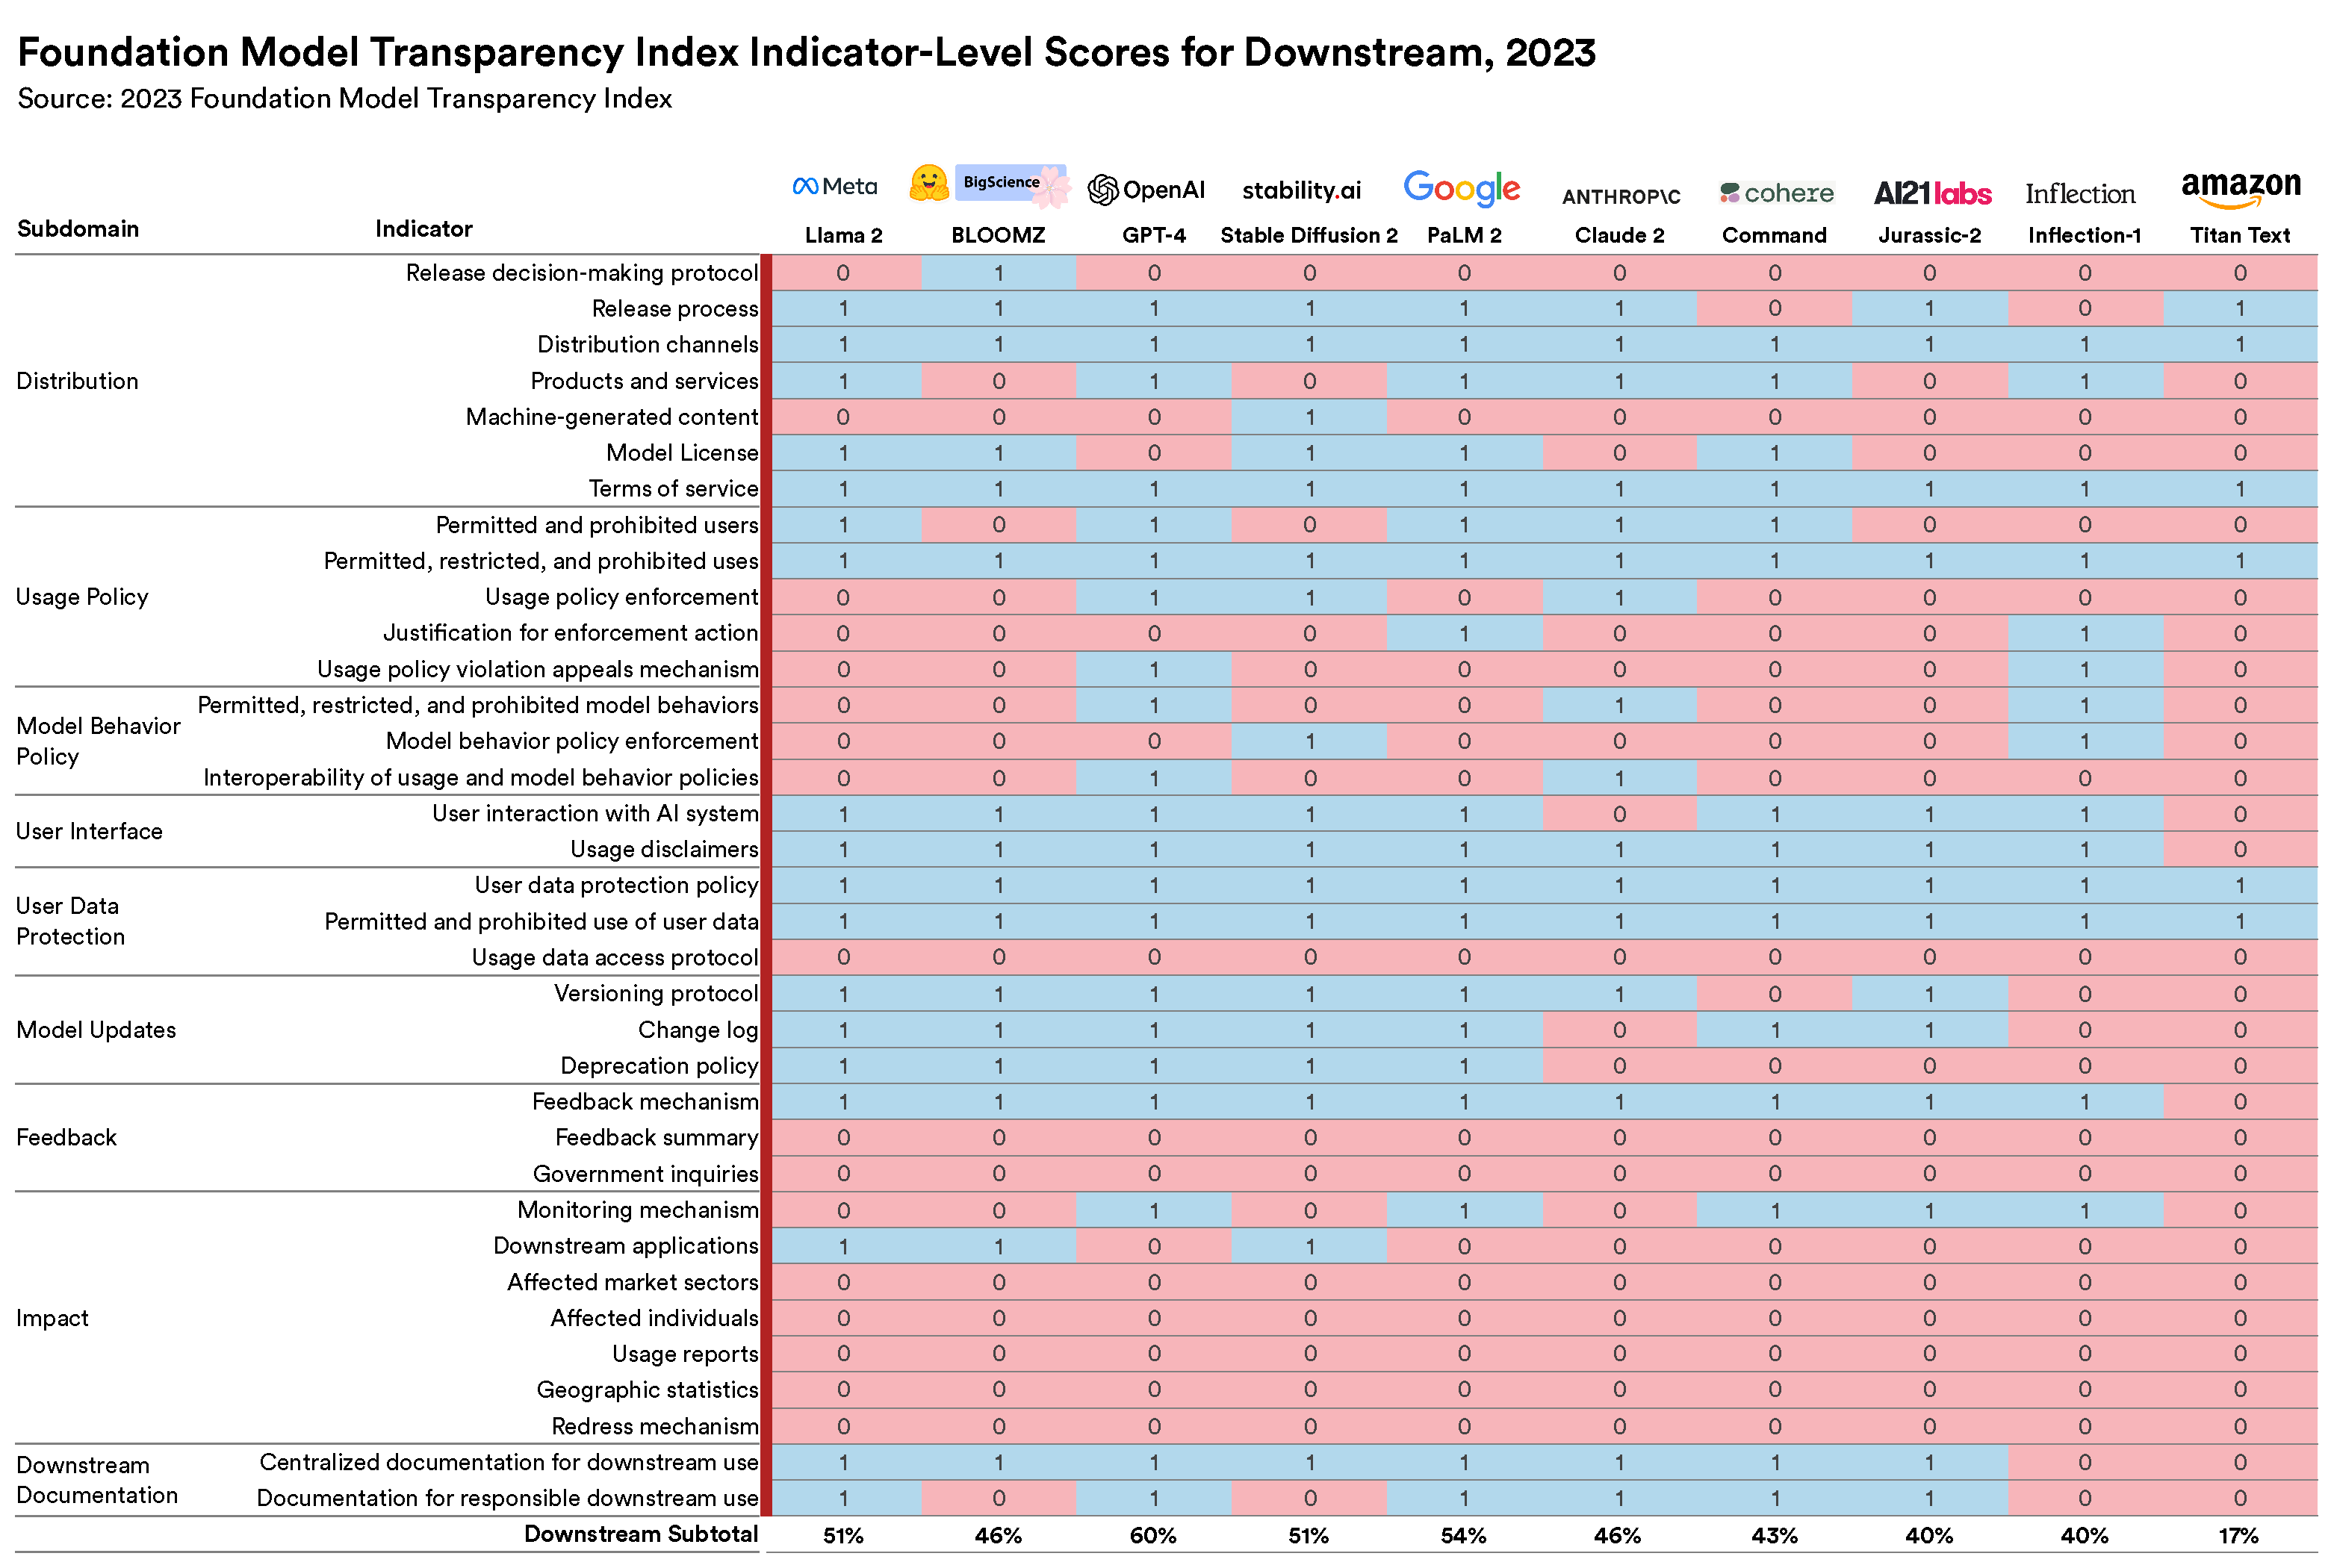
\includegraphics[keepaspectratio, width=0.85\pdfpagewidth]{figures/f12.pdf}
\end{minipage}
\caption{\textbf{Downstream Scores by Indicator.} 
The scores for each of the \numdownstreamindicators downstream indicators.
}
\label{fig:downstream-scores}
\end{figure}

\clearpage

% Revert to initial values
\eject
\pdfpagewidth=\originalwidth \pdfpageheight=\originalheight
\newgeometry{top=2cm, head=10pt, left=2cm, right=2cm,bottom=2cm}


\paragraph{Most model indicators are scored by some developer, though most developers score poorly on indicators related to evaluating intentional harms, mitigations, and inference efficiency.}
Of the 33 indicators in the model domain, at least one developer scores a point on 29 of them. 
Further, multiple developers score points on 27 model indicators.
The 4 indicators for which no developer scores points are (i) intentional harm evaluation, (ii) external reproducibility of mitigations evaluations, (iii) third party mitigations evaluations, and (iv) inference compute evaluation.
The 2 additional indicators for which only one developer scores points are limitations demonstration (\cohere) and external reproducibility of internal harm evaluation (\openai).
While many companies describe risks (including the risk of intentional harms), they do not share sufficient information related to evaluations of intentional harm or the reproducibility of evaluations of mitigations.
In the case of inference, we believe standards are needed akin to MLPerf \citep{reddi2020mlperf} to rigorously benchmark the inference of foundation models \citep{narayanan2023cheaply} given the key role of efficient inference and low latency in the usability of models \citep{lee2023evaluating}.
We see that \bloomz in particular provides a potential benchmark for language models by tracking the time spent for a fixed task (generating 100 tokens given a 7 token prefix) on fixed hardware (a NVIDIA A100-80GB GPU), though compute is not measured.\footnote{See \url{https://huggingface.co/blog/habana-gaudi-2-bloom}.}

\hypertarget{downstream-results}{\subsection{Downstream results}}
\label{sec:downstream-results}

Downstream indicators assess transparency regarding the use of foundation models, spanning subdomains related to distribution, policies constraining the use and behavior of the model, user interfaces, user data protection, model updates, feedback, impact, and documentation. 
Indicators in these subdomains characterize transparency related to how the foundation model is deployed and its downstream effects on the ecosystem and society. 
Our analysis is based on publicly available information about how the foundation model is distributed, how it can and cannot be used, how users can give feedback and seek redress, broader societal impacts, and the how the model affects actors downstream of the developer in the supply chain.
Here, we conduct a fine-grained analysis at the level of subdomains and indicators based on \reffig{downstream-scores}.

\paragraph{Downstream scores show less spread across developers.}
Total scores on downstream indicators are tightly clustered around the mean of 15.7 out of 35, which corresponds to 44.9\% of the \numdownstreamindicators downstream indicators. 
With the exception of \amazon (6 out of \numdownstreamindicators; 17.1\%), the other nine developers all score between 14 and 21 points.
The highest-scoring on the downstream domain is \openai at 21 points and the lowest-scoring (barring \amazon) are \aitwentyone and \inflection at 14 points.
In \refsec{correlations}, we clarify the extent to which these smaller margins in scoring discrepancies in the downstream domain are due to high agreement in indicator-level scores across companies.

\paragraph{\impact is the least transparent subdomain in the entire index.}
To clarify the downstream impact of a given foundation model, the \impact subdomain includes indicators on monitoring mechanisms, affected market sectors, affected individuals, usage reports, geographic statistics, and redress mechanisms.
Strikingly, the mean score across all developers on this subdomain is just 11\%, with 8 developers scoring points on just 1 of the possible 7 indicators and the remaining 2 scoring none of the indicators. 
No developer scores points on affected market sectors, affected individuals, usage reports, geographic statistics, or redress mechanism.
This means that there is essentially no information about how many people, sectors, and regions foundation models are impacting. 
\openai, \google, \cohere, \aitwentyone, and \inflection are the only developers to disclose a potential monitoring mechanism for tracking model use. 
And only open foundation model developers share limited information about downstream applications, whereas the rest provide no information.\footnote{We score the downstream applications indicator quite generously: all of the open developers score points because they discloses which Hugging Face "Spaces" are also using the model via Hugging Face's platform.
However, we emphasize that this is still a poor proxy for the number of applications dependent on the foundation model.} 

\paragraph{Developers are significantly more transparent about \distribution than other major dimensions of (downstream) transparency.}
Across the four major dimensions of transparency in the downstream domain (\distribution, \usagepolicy, \feedback, \impact), mean scores are on the higher end only for \distribution at 59\%, with the other three all below 50\%. 
Every developer shares information about distribution channels, or the pathways by which the model is made available to entities beyond the model developer organization.
Every developer provides terms of service that cover the distribution of its foundation model.\footnote{As with several downstream indicators, we assessed the terms of service of the primary distribution channel. For example, this meant that we assessed Microsoft Azure's terms of service for Meta.}
Most developers share information about their process for releasing their flagship model (8 of 10) as well as the developer's products and services that use the foundation model (6 of 10).
Half of developers share information about the license under which the model is distributed.
% Similarly, in terms of documentation, most developers provide centralized documentation to facilitate downstream use (80\%) and half provide documentation on responsible use.
% This gives some evidence that developers use transparency to coordinate with actors at different points in the supply chain, though we anticipate more robust coordination will be needed to address harms \citep{bommasani2023ecosystem, cen2023supplychain}.
% Some developers have continued to improve downstream documentation as they release new models \citep{bommasani2023eu-ai-act}, resulting in a marked improvement in transparency as evidenced by documents such as Meta's Llama 2 Responsible Use Guide. \footnote{See \url{https://ai.meta.com/llama/responsible-use-guide/}}

\paragraph{In spite of broad transparency on the \distribution subdomain, developers are highly opaque around release decisions.}
Within the \distribution subdomain, developers score poorly on the release decision-making protocol indicator; \huggingface is the only developer that shares information about its decision-making protocol for release.
Although there has been an extensive focus on release strategies in the literature on foundation models \citep{solaiman2019release, sastry2021release, shevlane2022structured, liang2022community-norms, liang2022condemning, solaiman2023gradient, widder2023open, seger2023open}, developers across the release spectrum share very little information about how and why they release their flagship models. 
In particular, we highlight that many of companies we assess have written about the broader topic of release, but not in a way that is precise to their specific decisions for their flagship models.\footnote{We note that following \informationfreezedate, \anthropic released information about its approach to responsible scaling: \url{https://www.anthropic.com/index/anthropics-responsible-scaling-policy}.}

\paragraph{\usagepolicy and \modelbehaviorpolicy subdomain scores are uneven across developers.}
Scores on the \usagepolicy subdomain are uneven, with all developers scoring points on the indicator for permitted, restricted, and prohibited uses, but only two (\openai and \inflection) scoring points on the usage policy violation appeals indicator.
This reflects the lack of industry standards regarding precisely how foundation model developers should restrict the use of their models. 
We found that different developers provide this information in different types of documentation, ranging from standalone Acceptable Use Policies to Content Policies to terms in the model license, and that many developers share some of this information in several different documents. 

While developers did provide some transparency on usage policies related to a user's obligations, they did not provide a similar level of transparency on the restrictions they place on their model's behavior. 
Scores on indicators in the \modelbehaviorpolicy subdomain were relatively weaker, with a mean across the 3 indicators of 23\% compared to 44\% for the 5 usage policy indicators.
\openai, \anthropic, and \inflection are the only developers who provide information about permitted, restricted, and prohibited model behaviors, while only \inflection and \stability provide information about how they might enforce such restrictions.
\openai and \anthropic are the only developers who make clear how their models are expected to behave in the event that a user violates the usage policy. 
In part, we believe the norms and standards around model behavior are rather immature, meaning that developers do not provide a clear conceptualization of if/how they impose a model behavior policy.
For example, the role of modeling decisions (\eg the use of reinforcement learning from human feedback or constitutional AI) on behaviors (\eg model refusals to specific requests) are not made clear.

\paragraph{Identical scores on the \dataprotection subdomain across all developers.}
For the \dataprotection subdomain, scores are uniform across developers, with every developer scoring points on user data protection policy, as well as permitted and prohibited uses of user data.
However, no developer scores points on usage data access protocol. 
This may reflect that few, if any, companies actually share usage data externally, meaning companies may perceive that the need to develop protocols for sharing such data is limited. 
However, developers' data protection policies include many provisions that would allow them to share such usage data, and specific protocols for how and when they do so are not transparent.

\paragraph{Developers lack transparency on the \feedback subdomain.} 
Developers score relatively poorly on \feedback indicators, scoring only 30\% of the available points. 
While every developer but \amazon has a public mechanism for collecting feedback on its model, none provide information such as a feedback summary or details on government inquiries, such as requests for user data (which social media companies disclose).
This is likely a function of how nascent the foundation model ecosystem is: companies have only been collecting feedback for a few years, and it took social media companies several years to respond to public calls for transparency around the feedback they receive from users and governments.
Moving forward, more robust transparency reporting practices that provide the public with more information regarding these forms of feedback will likely be necessary.\footnote{For example, consider the EU's DSA Transparency Database, implemented on the basis of the Digital Services Act to provide transparency on content moderation decisions: \url{https://transparency.dsa.ec.europa.eu/}.}

\paragraph{Developers are fairly transparent on the \updates subdomain.}
5 of 10 developers provide clear information about their versioning protocol, change log, and deprecation policy.
\inflection and \amazon, however, score zero points on these indicators, which may be due in part due to the face that \inflectionone and \titan are at an earlier stage of release than some other flagship models. 
While there is a wide variation in the type, specificity, and quality of documentation provided related to \updates, as with other indicators, we assess these metrics generously and allocate points on the basis of transparency alone. 

\paragraph{Developers score well on the \interface subdomain, though this may change due to deployments on mobile phones.}
Developers scored highly on \interface indicators (average score of 85\%), with more than half of developers scoring points on both indicators, which assess if users are told they are interacting with an AI system and if users are provided appropriate disclaimers. 
Developers frequently disclose to users that they are interacting with a specific foundation model by including the name of the foundation model somewhere in the user interface, while they give usage disclaimers upon sign-up for the user interface via a link to the terms of service or usage policy. 
Unlike all other indicators, we generally had to make use of step 7 in the and directly interact with developers' models via a user interface to assess these indicators. 
However, \amazon did not have a publicly available user interface in advance of \informationfreezedate, meaning that it could not receive these points. 
We initially assessed transparency of deployments on mobile devices in some cases, though we ultimately did not consider these deployments for scoring.
With that said, we highlight that the same standard for transparency of user interfaces does not currently appear to be met by mobile deployments from \openai and \inflection.
Overall, we believe in the importance of providing transparency through user interfaces as it can help foundation models avoid the formation of the "dark patterns" we have seen develop with other digital technologies \citep{10.1145/3359183}.
For example, we highlight that \anthropic does not make clear that a user is interacting with an AI system, except for the textual description "Message Claude."

\hypertarget{release-results}{\subsection{Results for open and closed developers}} \label{sec:release-results}
\begin{figure}
\centering
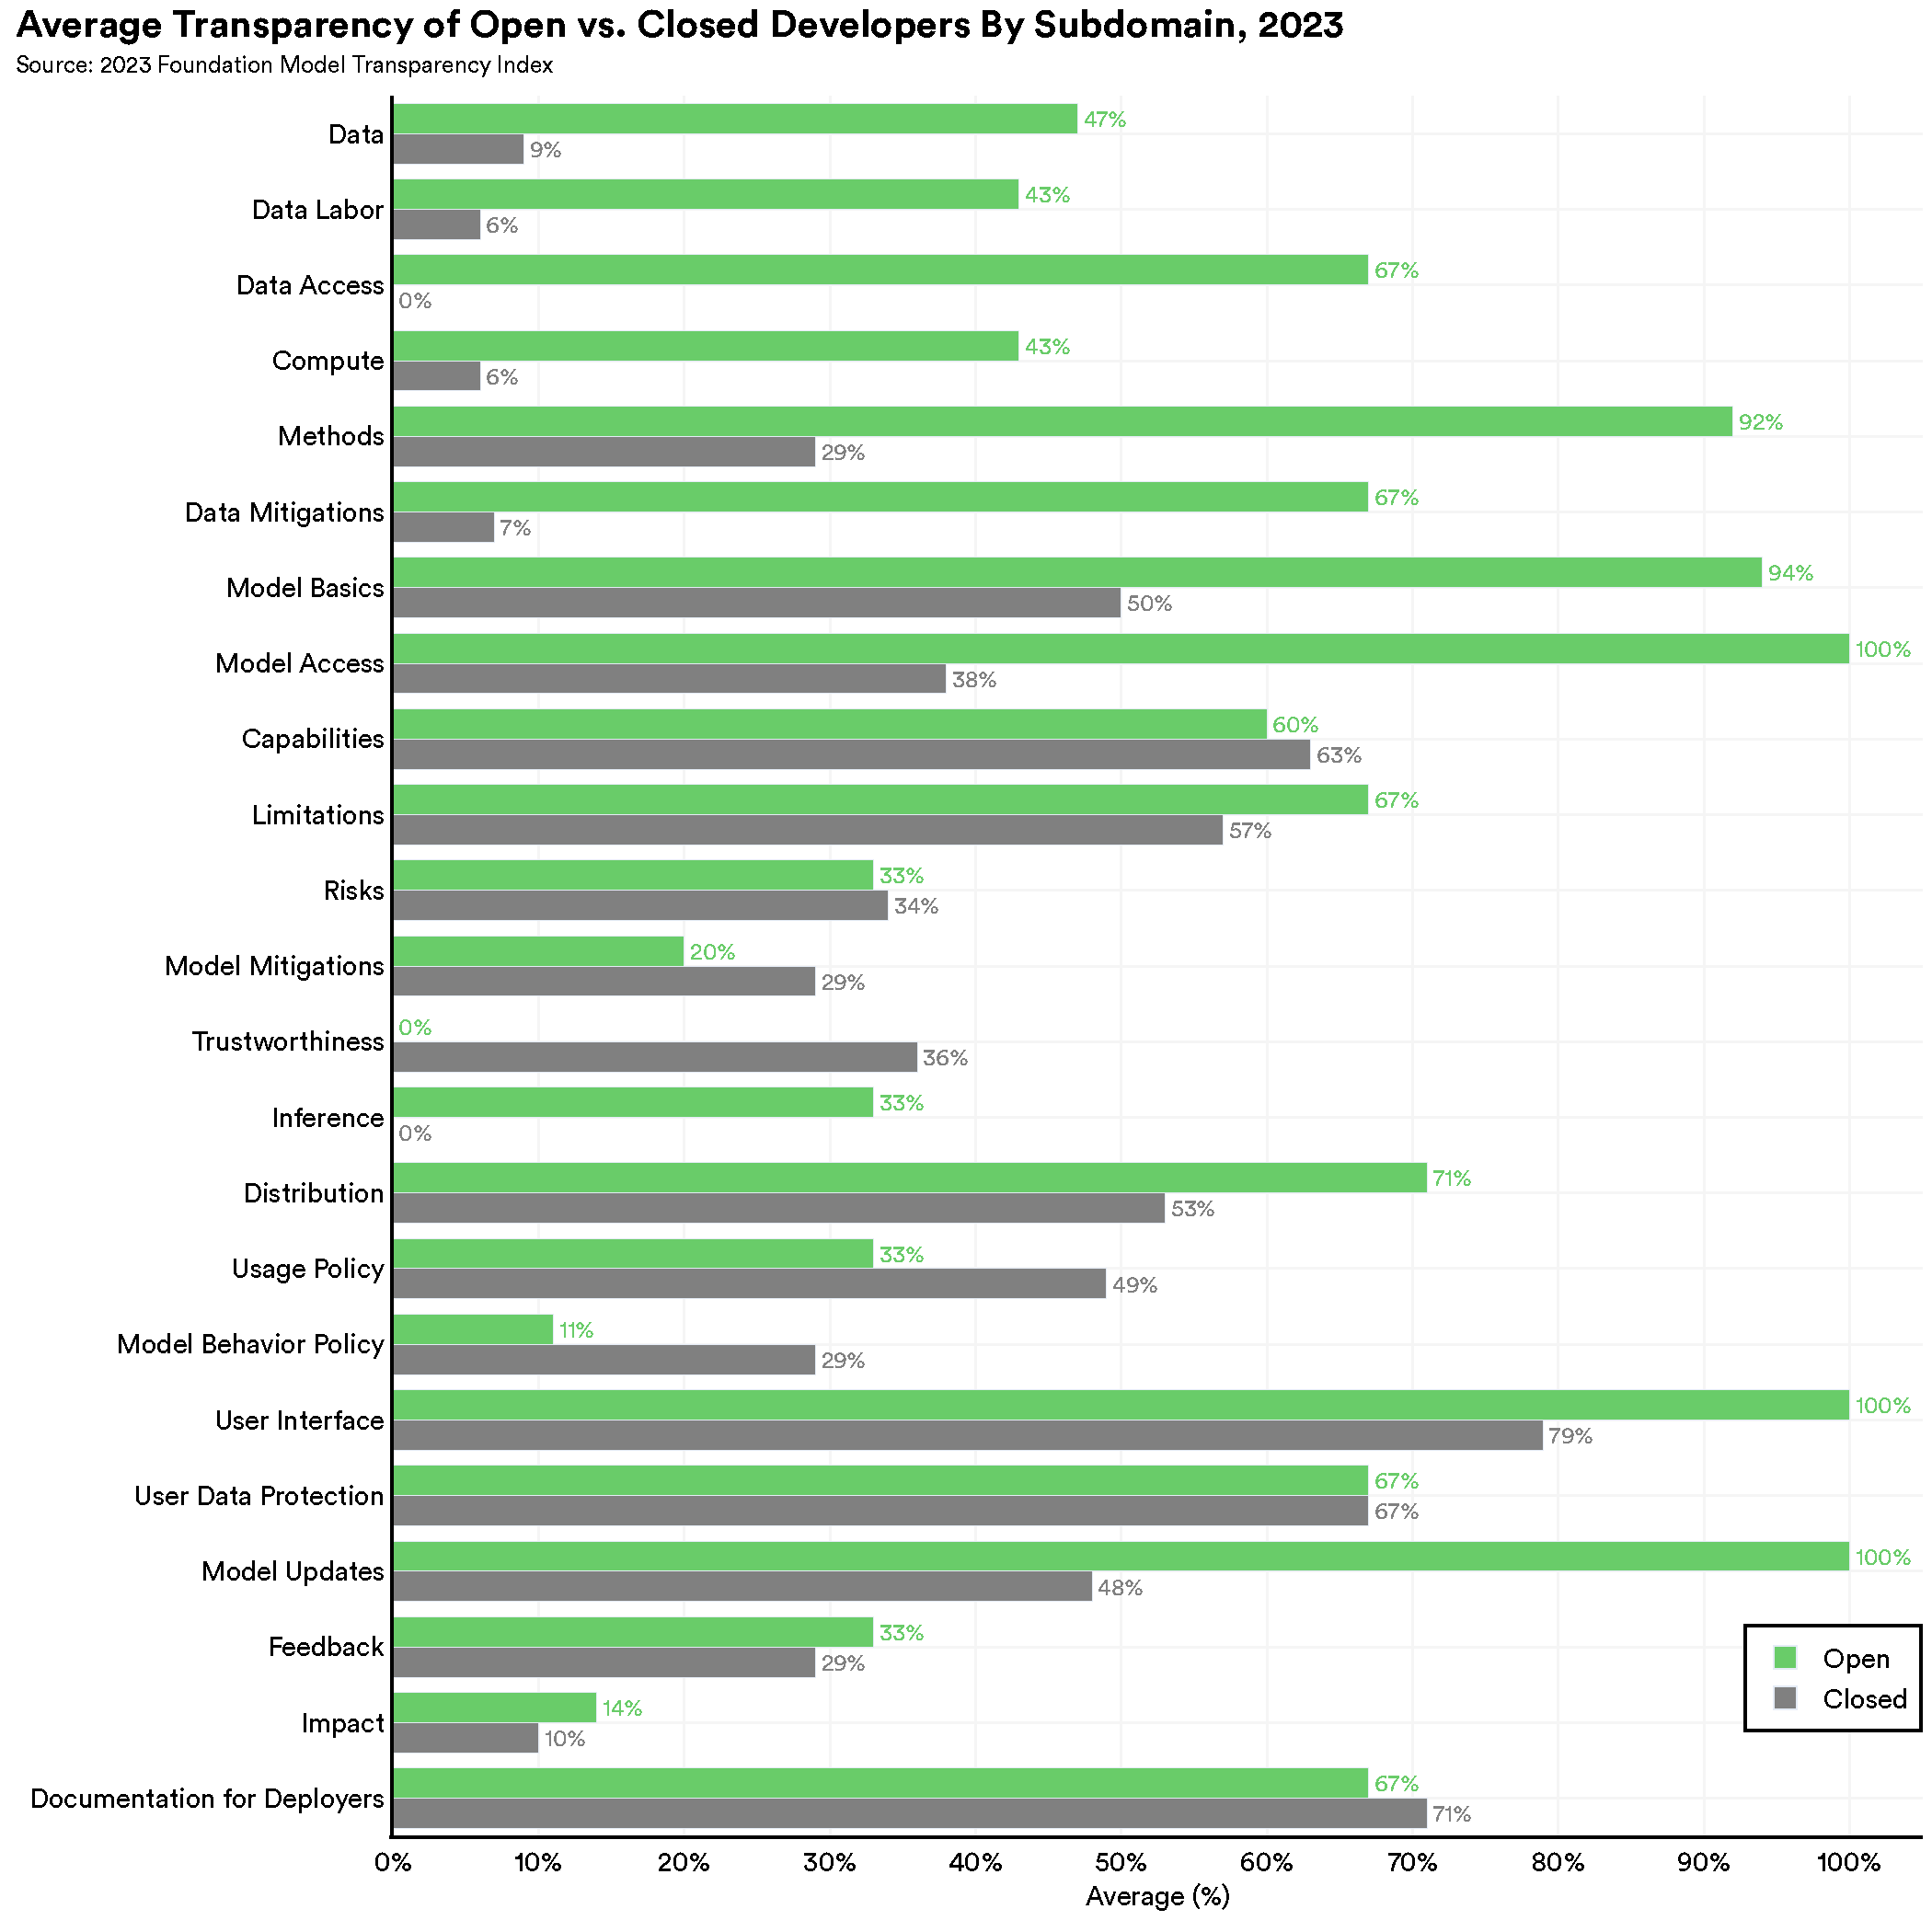
\includegraphics[keepaspectratio, height=\textheight, width=\textwidth]{figures/f13}
\caption{\textbf{Open vs. Closed by Subdomains.} 
The mean score for the 3 open developers (\meta, \huggingface, \stability) and the 7 closed developers (\openai, \anthropic, \google, \cohere, \aitwentyone, \inflection, \amazon) across each of the 23 subdomains. Note: the number of indicators per subdomain varies widely.
}
\label{fig:open-closed}
\end{figure}


Foundation models are released by different developers using a variety of release strategies \citep{liang2022community-norms, solaiman2023gradient}.
In particular, we deliberately chose several developers that are more \textit{open} (\eg release the weights of their model, perhaps along with the data used to build the model)and others that are more \textit{closed} (\eg only provide access via an API).
The topic of release and the (reductive) dichotomy of open vs. closed has emerged as a primary topic of technical and policy research on foundation models \citep{solaiman2019release, sastry2021release, shevlane2022structured, liang2022community-norms, liang2022condemning, solaiman2023gradient, widder2023open, seger2023open}.
To clarify how transparency differs between the open developers we assess (\ie \meta, \huggingface, \stability) and the closed developers (\ie \openai, \google, \anthropic, \cohere, \aitwentyone, \inflection, \amazon), we emphasize the distinction in \reffig{open-closed}. 

\paragraph{Open developers score higher in aggregate and on every domain.}
We establish a clear trend that the open developers score higher overall, with all three being among the four highest-scoring developers (see \reffig{overall-scores}).
In particular, every open developer is nearly at least as transparent in terms of aggregate score as the highest-scoring closed developer (\openai): \meta and \huggingface are at least 5 points higher, and \stability is within a point of \openai.
Further, this trend is established more strongly through domain-level analysis, where open developers score higher on average than closed developers across all domains (\ie upstream, model, downstream).
The mean score of open developers on upstream indicators is 53\% compared to 9\% for closed developers, 51\% for open developers on model indicators compared to 39\% for closed developers, and 49\% on downstream indicators compared to 43\% for closed developers.
To ensure these trends are robust to outliers, we highlight that the trends hold even when considering medians instead of means (upstream: 50\% to 9\%, model: 48\% to 45\%, downstream: 51\% to 43\%).

We emphasize that our findings confirm common hypotheses that open developers will in general be more transparent with respect to the upstream resources required to build their models (which also aligns with some making the data they use publicly available), but our findings dispute hypotheses that open developers will be less transparent on downstream matters due to their weaker control over downstream use.
While we believe that closed developers providing APIs are better positioned to collect information on the downstream use of their models, in practice these developers do not disclose this information to provide greater public transparency.

\paragraph{Open developers score higher on most subdomains.}
Open developers score higher than closed developers on 15 of the \numsubdomains subdomains, which account for 68 of the 100 indicators. 
The mean score of closed developers is higher than that of open developers on indicators in the subdomains of \capabilities, \risks, \modelmitigations, \trustworthiness, \usagepolicy, \modelbehaviorpolicy, and \documentation.
We highlight that these seven subdomains point to two broader themes: closed developers in some cases may be higher-resourced or face stronger incentives to proactively address certain matters around responsible AI (\eg \risks, \modelmitigations, \trustworthiness).
In addition, closed developers often have a closer coupling between the foundation model we assessed and downstream services, meaning that certain user-related aspects of transparency are potentially of higher priority (namely the \usagepolicy). 
For example, many closed developers provide products built on top of their flagship foundation model, providing users of their platforms and clients who license their proprietary foundation models with an opportunity to push for transparency.

The mean score of open developers is higher than closed developers on every upstream subdomain, with major score differentials especially for the \data, \compute, and \methods subdomains.
Looking at the difference in average scores by release strategy, we see large disparities in favor of open models in each domain, with the largest gaps for \dataaccess (67\% to 0\%), \methods (92\% to 29\%), and \datamitigations(67\% to 7\%).
We also observe similar large differentials (40\%+) for \modelbasics, \modelaccess, and \updates.
While less stark, we highlight the superior transparency on average for the \distribution subdomain as especially surprising given that closed developers maintain greater control over distribution by virtue of being closed.

\paragraph{Indicator-level analysis further demonstrates the disparity between open and closed developers.}
At the indicator level, the median open developer outscores the median closed developer on 28 indicators (18 upstream, 7 model, 3 downstream), while the median closed developer scores higher on just 6 indicators (0 upstream, 2 model, 4 downstream). 
The median open developer and the median closed developer both score points on 22 indicators and neither scores points on 44 indicators. 

\paragraph{The open developers we assessed provide greater transparency than their closed counterparts.}
Overall, each level of analysis points in the same direction: open developers are reliably more transparent.
In particular, we highlight that the release of assets (\eg model weights, data, code) may be significantly underweighted in terms of its broader transparency effects.
Our findings dispel the belief that closed developers are more likely to be transparent about downstream matters due to their greater control over deployment, while emphasizing that both open and closed developers continue to be extremely opaque in terms of the downstream impact of their foundation models.
With this in mind, we caution that our assessment is necessarily based on the practices of some of the highest-resourced open and closed developers, so these trends should not be taken as sufficient evidence to claim that all open developers are more transparent than closed developers.
And we believe there is ample opportunity for closed developers to address these gaps in transparency as we discuss in \refsec{recommendations-developers}.

\hypertarget{correlations}{\subsection{Correlations between companies}}
\label{sec:correlations}
\begin{figure}
\makebox[\textwidth][c]{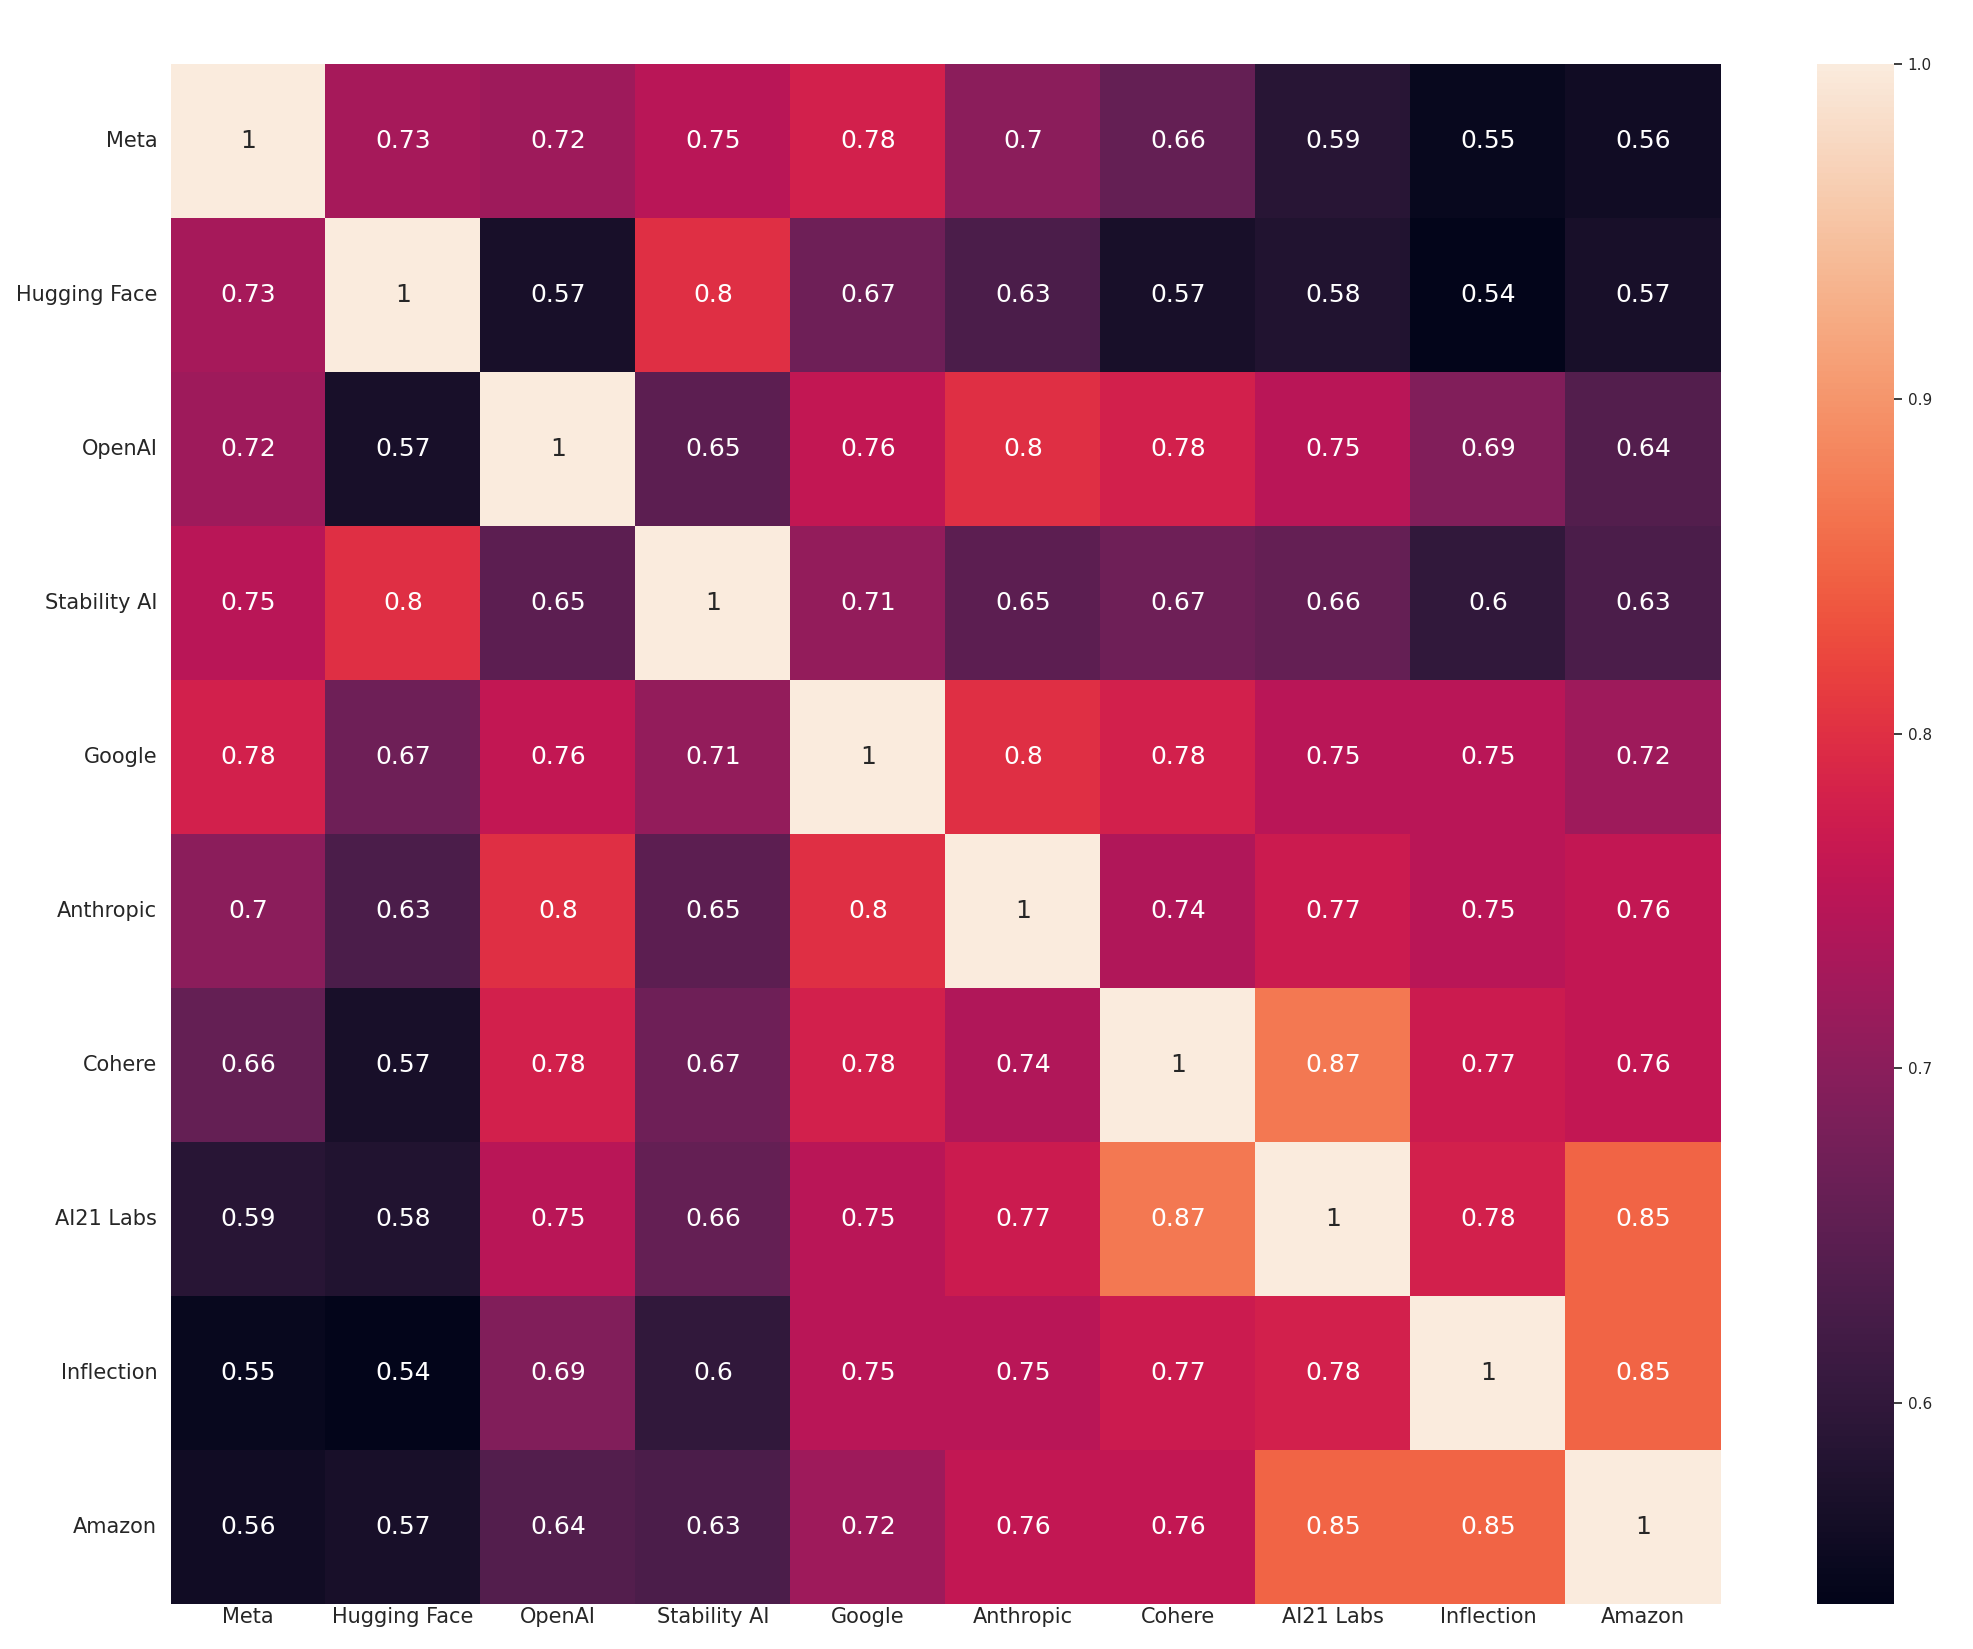
\includegraphics[keepaspectratio, width=1.25\textwidth]{figures/all_company_correlations.png}}
\caption{\textbf{Correlations between Companies.} The correlation between the scores for pairs of companies across all indicators. Correlation is measured using the simple matching coefficient (\ie agreement rate), which is the fraction of all indicators for which both companies receive the same score (\ie both receive the point or both do not receive the point).
}
\label{fig:overall-correlations}
\end{figure}
\paragraph{Measuring correlations.}
The \numindicators $\times$ \numcompanies scores introduces data-driven structure.
In particular, it clarifies relationships that arise in practice between different regions of the index.
Here, we consider the \textit{correlations}, in scores, focusing on company-to-company similarity for simplicity.
For example, if two companies receive similar aggregate scores, is this because they satisfy all the same indicators or do they score points on two very different sets of indicators?

In \reffig{overall-correlations}, we plot the correlation between every pair of companies.
To measure correlation, we report the simple matching coefficient (SMC) or the agreement rate.
The SMC is the fraction of the \numindicators indicators for which both companies receive the same score (\ie both receive a zero or both receive a 1). 
As a result, a SMC of 0 indicates there is no indicator such that both companies receive the same score and a SMC of 1 indicates that for all indicators both companies receive the same score. 
For this reason, the correlation matrix is symmetric and guaranteed to be 1 on the diagonal. 

To systematically analyze the results, we consider three patterns in the correlation matrix:
(i) individual cells with very small or very large values (\ie highly similar or highly dissimilar company pairs),
(ii) individual rows with consistently small, consistently large, or highly varied values (\ie unusual companies),
and
(iii) structural patterns across the correlation matrix.

\paragraph{Strongly correlated company practices.}
In terms of the most correlated company pairs, we identify a few regions of the correlation matrix.
First, we identify the three most correlated pairs: 
(\cohere, \aitwentyone; SMC = 0.87),
(\aitwentyone, \amazon; SMC = 0.85),
and
(\inflection, \amazon; SMC = 0.85).
These pairs are all among the four lowest-scoring companies, though we note the inclusion of \cohere is interesting given \cohere's overall score (34) is closer to the average (37) and the middle-scoring group of companies (\ie including \google and \anthropic).
In addition to these pairs, if we consider the other highly-correlated pairs (SMC $\geq$ 0.8), we identify:
(\huggingface, \stability; SMC = 0.80),
(\openai, \anthropic; SMC = 0.80),
and
(\google, \anthropic; SMC = 0.80).
In particular, we observe that the company correlations identify clear structure: \huggingface and \stability are the only two developers to release both data and models openly, and the trio of \openai, \google, and \anthropic are the three members of the Frontier Model Forum that we assess.

\paragraph{Weakly correlated company practices.}
In contrast, we see that the least correlated pairs (SMC < 0.6) are pairs involving \meta and the three lowest-scoring developers as well as pairs involving \huggingface and five of the seven closed developers (\openai, \cohere, \aitwentyone, \inflection, \amazon).
These are all pairings between an open and a closed developer.
More broadly, we highlight that \meta is the sole developer that is not correlated with SMC at least 0.80 with any other developer, with the most similar other developer being Google at 0.78 (see below for further analysis). 
This means \meta is rather unique in terms of the indicators where it scores points; it is the sole developer that is not strongly correlated with any other company, even including the two other open developers.
Nevertheless, the least correlated pair of companies still agrees in over half the indicators (SMC = 0.54), which is not surprising given that all the companies are opaque (\eg if all the companies all scored 0 on every indicator, they would necessarily be perfectly correlated with SMC = 1).

\begin{figure}
\makebox[\textwidth][c]{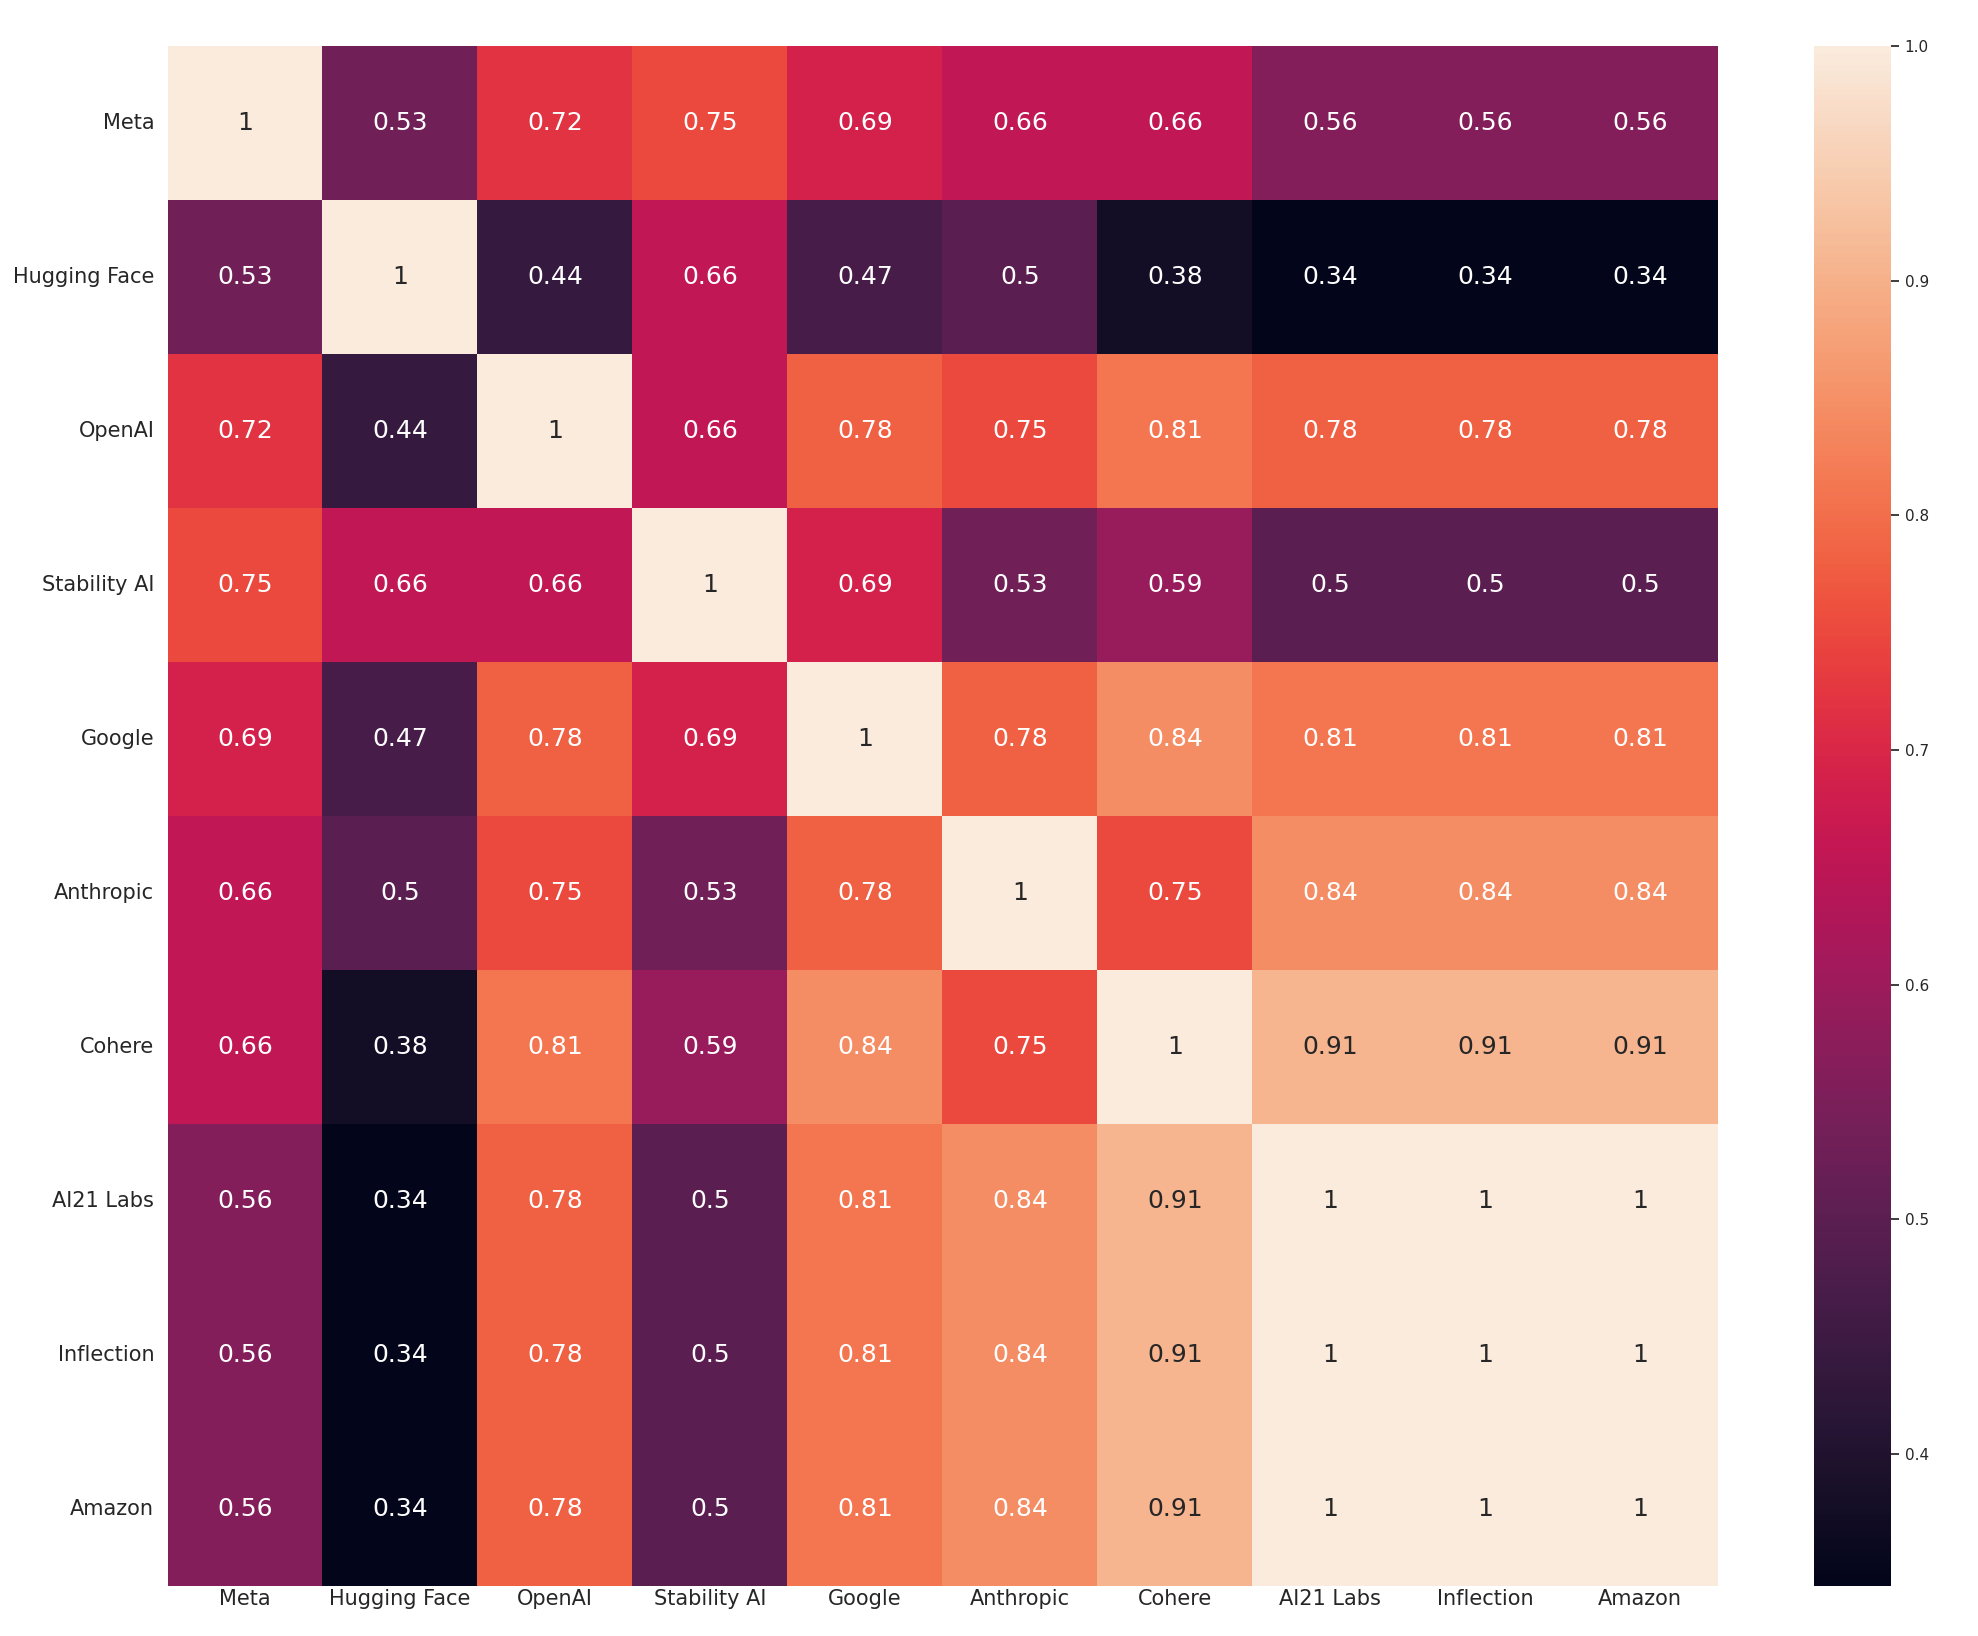
\includegraphics[keepaspectratio, width=1.25\textwidth]{figures/upstream_company_correlations.png}}
\caption{\textbf{Correlations between Companies (Upstream Indicators).} The correlation between the scores for pairs of companies across all indicators when only considering upstream indicators. Correlation is measured using the simple matching coefficient (\ie agreement rate), which is the fraction of all indicators for which both companies receive the same score (\ie both receive the point or both do not receive the point).
}
\label{fig:upstream-correlations}
\end{figure}

\paragraph{Upstream correlations.}
In \reffig{upstream-correlations}, we plot the correlation between every pair of companies when considering only indicators from the upstream domain.
Since the four lowest-scoring companies overall also score zero (or near-zero in the case of \cohere) points on the upstream indicators, they are necessarily extremely correlated.
For the same reason, the extent to which the remaining six companies are correlated with the three lowest-scoring companies is precisely proportional to their own opacity on the upstream domain.
Looking at the three companies that score in the middle overall (\google, \anthropic, \cohere), we see their indicator-level transparency is reasonably correlated.
We also see a similar trend where \openai, \google, and \anthropic are correlated, though in this case \openai and \cohere are even more correlated with an SMC of 0.81.
Interestingly, while the three open developers score much higher overall than any of the seven closed developers for the upstream domain, the correlations between them are somewhat different than in the other domains: there is a weaker correlation between \huggingface and \stability, and \meta's correlation with \openai and \stability is stronger than its correlation with \huggingface.
Despite the fact that \meta and \huggingface are the two highest-scoring companies on upstream, they are not especially correlated (SMC = 0.53) in that domain.
These discrepancies coincide with the indicators where \huggingface scores points and the other two open developers (\meta, \stability) do not, namely those relating to data sources and data labor. 
Given the large spread in scores across developers in the upstream domain, we see the related effect that the correlations can be quite variable with some at or near 1 and others well below 0.5 (minimum upstream SMC = 0.34).

\begin{figure}
\makebox[\textwidth][c]{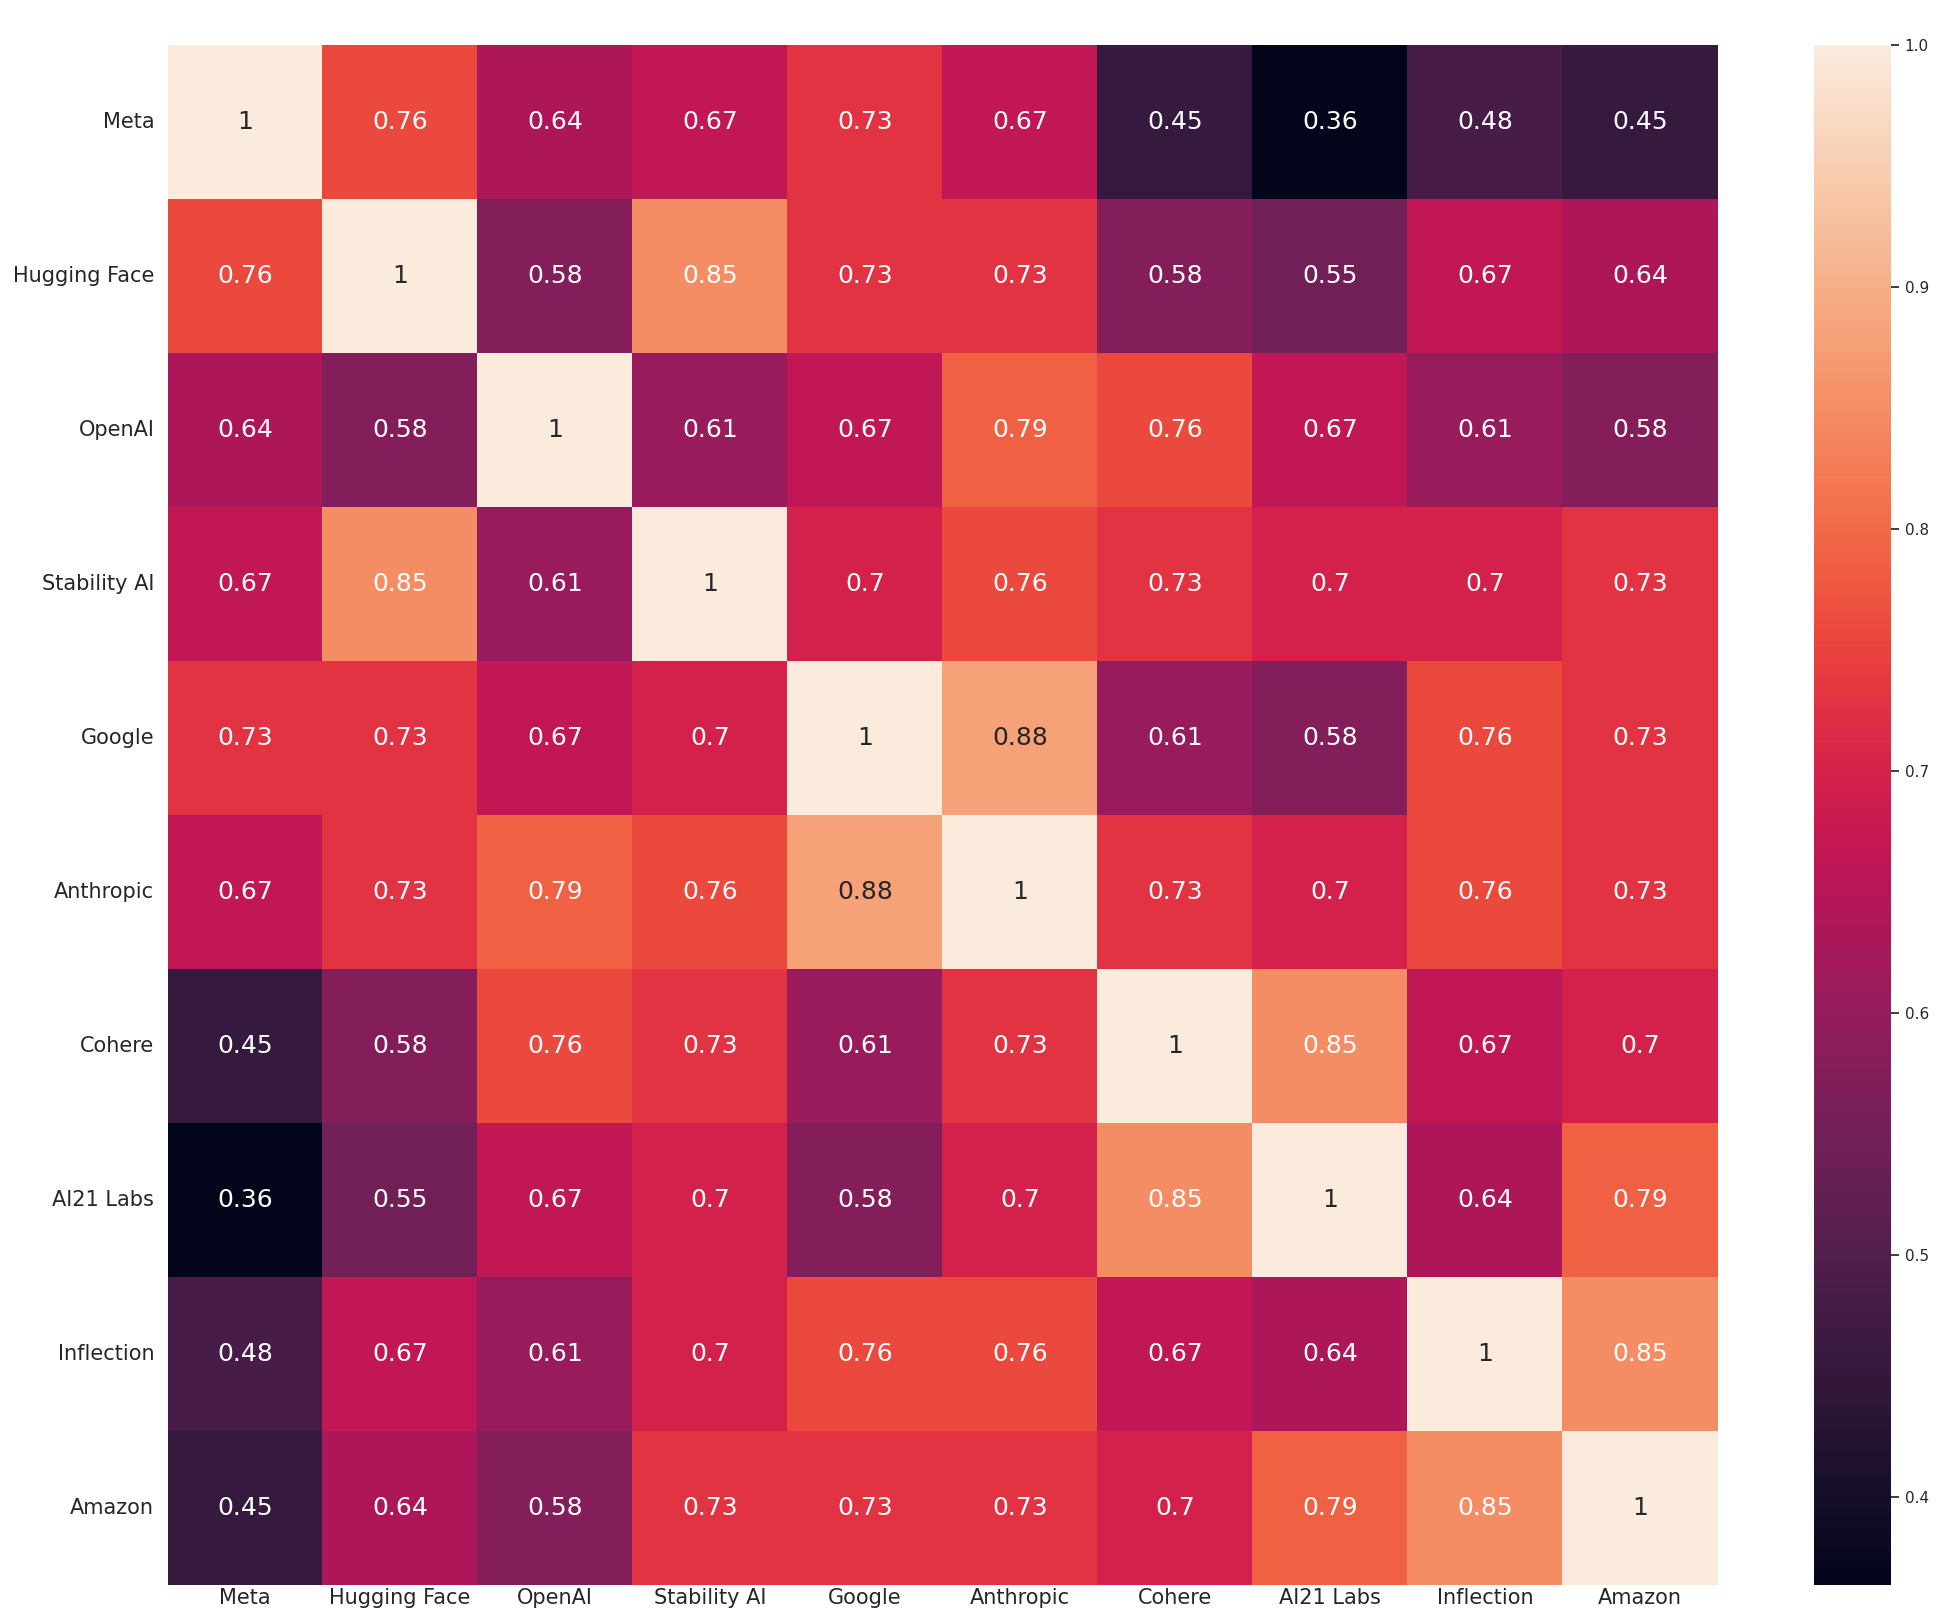
\includegraphics[keepaspectratio, width=1.25\textwidth]{figures/model_company_correlations.png}}
\caption{\textbf{Correlations between Companies (Model Indicators).} The correlation between the scores for pairs of companies across all indicators when only considering model indicators. Correlation is measured using the simple matching coefficient (\ie agreement rate), which is the fraction of all indicators for which both companies receive the same score (\ie both receive the point or both do not receive the point).
}
\label{fig:model-correlations}
\end{figure}

\paragraph{Model correlations.}
In \reffig{model-correlations}, we plot the correlation between every pair of companies when considering only indicators from the model domain.
In contrast to the upstream correlations, we see a much more varied picture.
First, much like the overall correlations, we see strong correlations for (\cohere, \aitwentyone; SMC = 0.85) and (\inflection, \amazon; SMC = 0.85) but not necessarily for the other pairs between these four companies. 
Among the three Frontier Model Forum companies, we see a very strong correlation of 0.88 between \google and \anthropic, a fairly high correlation of 0.79 between \openai and \anthropic, but a considerably lower correlation for the third pair of \openai and \google at 0.67.
These trends, where \anthropic is highly correlated with both, but \openai and \google are not necessarily correlated, mirror what we observe for the overall correlations.
Similar to what we observed for the overall correlations, \huggingface and \stability are quite correlated as well with a correlation of 0.85, and \meta is not particularly correlated with any company (the highest is \huggingface at 0.76).


\begin{figure}
\makebox[\textwidth][c]{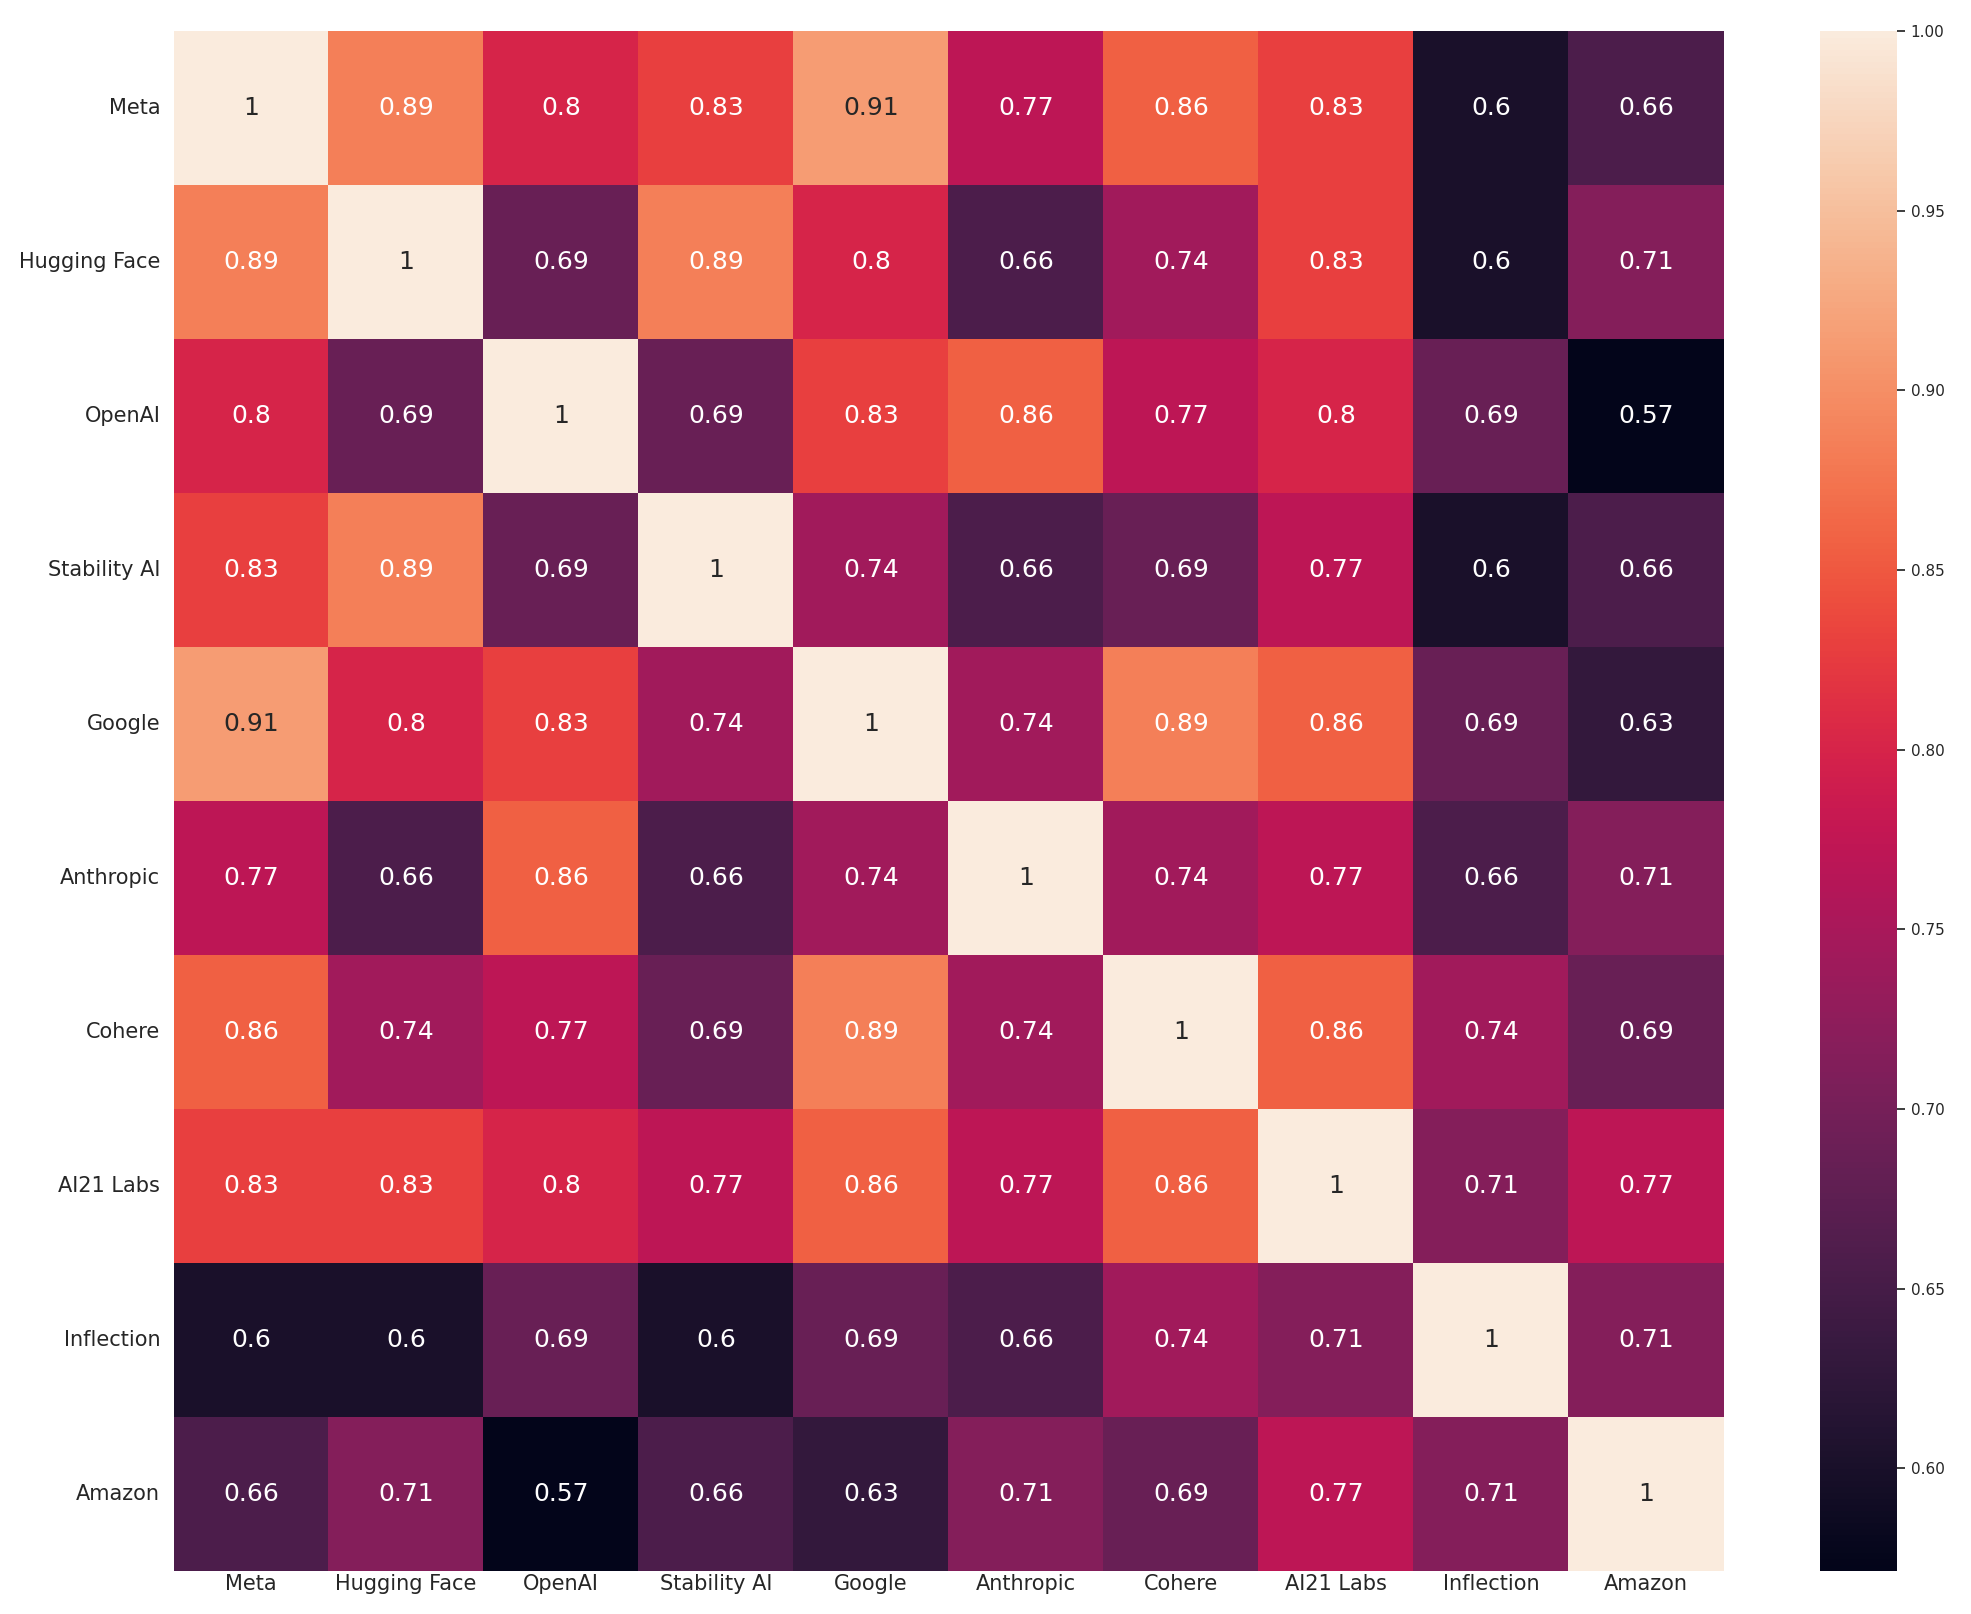
\includegraphics[keepaspectratio, width=1.25\textwidth]{figures/downstream_company_correlations.png}}
\caption{\textbf{Correlations between Companies (Downstream Indicators).} The correlation between the scores for pairs of companies across all indicators when considering only downstream indicators. Correlation is measured using the simple matching coefficient (\ie agreement rate), which is the fraction of all indicators for which both companies receive the same score (\ie both receive the point or both do not receive the point).
}
\label{fig:downstream-correlations}
\end{figure}

\paragraph{Downstream correlations.}
In \reffig{downstream-correlations}, we plot the correlation between every pair of companies when considering only indicators from the downstream domain.
The downstream correlations surface considerably different trends from the overall correlations or those for the other two domains.
In particular, we first highlight that \meta is strongly correlated with \google in their scores on downstream indicators.
Given that several of the downstream indicators related to broader corporate practices, the similarities between these companies may contribute to this result, though both companies are not strongly correlated with \amazon, the other Big Tech company we assess.
Relatedly, we see fairly strong correlations between \openai and \anthropic, which again may relate to their fairly similar business practices mapping onto specific downstream indicators (\eg indicators in the \modelbehaviorpolicy subdomain).
On the other hand, akin to the upstream subdomain, we see that \inflection is especially dissimilar from all of the open model developers (\meta, \huggingface, \stability). 
And, unlike the other correlation matrices, \openai and \amazon are more dissimilar than usual. 
Overall, while we do not observe it as clearly in the other correlation analyses, here we see all three pairs of open developers are highly correlated:
(\meta, \huggingface; SMC = 0.89),
(\meta, \stability; SMC = 0.83),
(\huggingface, \stability; SMC = 0.89).
This may reflect that all open developers have shared transparency challenges on specific indicators within the downstream domain (\eg monitoring mechanism and model behavior policy enforcement), perhaps stemming from the weaker control they have over downstream use. 
Overall, we find the complex structure and heterogeneity in the correlation for the downstream domain especially intriguing, given the aggregate scores for this domain are the most tightly clustered (see \refsec{downstream-results}).
That is to say, disaggregated indicator-level analysis is especially revealing for this domain compared to domain-level analysis.
